%talk about CVNNV, generally homorganic CC sequence
\chapter{Phonology Outline}
\label{sec:chap-phono}


\section{Introduction}
\label{sec:intro-phono}

This section presents a brief outline of Chakali phonology. An inventory
of phonetic and phonemic vowels and consonants, the syllable
structures, the phonotactics and the suprasegmentals are introduced.  The
presentation is intended
to provide evidence for the analytical choices.  The description
makes use of the International Phonetic Alphabet (IPA)  symbols to represent the
sounds
of the language. These should not be confused with the same IPA symbols used to 
represent  sets of phonological features, i.e.  distinctive feature bundles.
This domain representation mismatch is usually resolved by containing phonemes
and underlying representations within slash brackets  (e.g. {\I
/kæt/} `cat')  and  speech sounds and surface forms within square brackets (e.g.
{\I
[kʰæʔ]} `cat'). The former is a postulation and an abstraction,
while the latter  represents either the output of
phonological computation or the utterance as perceived by the linguist.  For the
rest
of this
exposition, if a Chakali expression is presented without the slash or  square
brackets, it should be interpreted as a broad phonetic
transcription.  The dash symbol (-) is
used to identify the edges of morphological units (e.g. kæt-s `cats'),  while 
the hash symbol (\#) separates word units.\footnote{Abbreviations are
listed on page \pageref{sec-ABB}. Other symbols used in this chapter are 
$]$ which identifies an
affix/stem/root boundary,  $]_{wb}$  a word boundary,   $]_{\sigma}$  a
syllable  boundary, and  \#\#  a strong boundary, e.g.
% an
utterance-final boundary. In the rule format,   the material following / 
represents the context,  and \_ is the position of the feature/segment in
question. The symbol C* indicates a condition where any number
of consonant (usually zero, one or two) can occur. A prose translation is given
for each rule.}  The parts of speech
of  Chakali expressions are provided: on one hand,  having the  information
on the part
of speech avoids ambiguity since the English gloss is often inadequate. On the
other hand,  it assists the search for phonological behaviour conditioned by
lexical category. The examples used as evidence in this section are all
presented in the lexicon in chapter \ref{sec:LEX-lexicon}. 
 

 
%(see section \ref{sec:lexicon})


\section{Segmental Phonemes Inventory}
\label{sec:seg-phon-invent}

The goal is  to identify the segmental phonemes of Chakali and their contrasts
by determining the phonetic properties in minimal contexts of speech sound
patterns.  Some
near-minimal pairs may appear, but the   majority of the evidence provided is
based on  minimal pairs. The vowels are examined first, followed by the
consonants. The set of (articulatory) features proposed in
\cite{Lade07} is assumed.

\subsection{Vowels}
\label{sec:vowels}

Chakali is treated as a language with nine underlying vowels and eleven
surface vowels. They
are presented in figure \ref{fig:Phon-phon-srf} in  vowel diagrams. Their
position is not the result of qualitative measurement. The surface vowels  [ɑ]
and  [ə] are discussed  at the end of this section. 


\begin{figure}[!htb]
\centering

\subfloat[Vowel Phonemes]{
\begin{tabular}{ccc}

 \begin{vowel}[simple]
\putcvowel{i}{1}
\putcvowel{e}{2}
\putcvowel{ɛ}{3}

\putcvowel{ɔ}{6}
\putcvowel{o}{7}
\putcvowel{u}{8}

\putcvowel{ɪ}{13}
\putcvowel{ʊ}{14}
\putcvowel{a}{4}
\end{vowel}
\end{tabular}
}
\qquad
\subfloat[Surface Vowels]{

 \begin{tabular}{ccc}


\begin{vowel}[simple]
\putcvowel{i}{1}
\putcvowel{e}{2}
\putcvowel{ɛ}{3}
\putcvowel{ɑ}{5}
\putcvowel{ɔ}{6}
\putcvowel{o}{7}
\putcvowel{u}{8}
\putcvowel{ə}{11}
\putcvowel{ɪ}{13}
\putcvowel{ʊ}{14}
\putcvowel{a}{4}
\end{vowel}


 \end{tabular}

}

\caption{Vowel phonemes and surface vowels in Chakali \label{fig:Phon-phon-srf}}
\end{figure}



Each vowel is presented below with minimal contrasts to motivate their phonemic
status.   Two sounds are contrastive if interchanging the two can change the
meaning of the word. The vowels are presented in opposition for their height,
roundness, backness and tongue root properties. Since Chakali does not show any
contrast of roundness and backness in the non-low vowels, roundness and backness
  are put together in the description under a {\sc robk} feature. The tongue
root
distinction, often identified either as a tense and lax distinction, or as a
close and open one,  is gathered under the feature {\sc atr} (i.e. advanced
tongue root). Low, mid and high are treated under {\sc height} in the
subsequent tables, but are captured in the summary table \ref{tab:featspec}
with the features {\sc hi}, {\sc mid}  and {\sc lo},  and the feature values +
and -. 


\newpage

\paragraph{Close front unrounded {\S i}}
\label{sec:i-phon-vowel}
The vowel [{\I i}] is perceived as front, unrounded, high and tense. 
\begin{center}
\begin{Itabular}{llll}
\Hline
Contrast &   cli. example & Gloss & PoS\\[1ex] \hline
{\sc height}	& zíŋ 	&	tail	& n\\	
	& záŋ &	rest area	& n\\
%	tʃítʃí  &cockroach sound &	ono\\
%	&	tʃítʃà&	teacher & n\\	
	&	bíí	&	seed	& n\\
	&	bìé	&	child	& n\\[0.5ex] \hline


{\sc robk}    &	dɪ́ɪ́l	&	inhabitant	& n\\
	&	dúl	&	right (side)	& qual\\		
	&	kísì &  pray & v\\
	&	kùsì & unable &  v\\[0.5ex] \hline
	

{\sc atr}  	& ɲìŋ́ &  sore  & n\\
    &  ɲɪ́ŋ &   tooth & n\\
	& dì	&	eat	&	v\\
	& dɪ̀    &	if	&		conn\\
\Hline
\end{Itabular}
\end{center}


\paragraph{Near close near front unrounded {\S ɪ}}
\label{sec:I-phon-vowel}
The vowel [{\I ɪ}] is perceived as front, unrounded, high and lax. 
\begin{center}
 \begin{Itabular}{llll}
\Hline
Contrast &   cli. example & Gloss & PoS\\[1ex] \hline

{\sc height}  & 	mɪ́ŋ	&	I		&	1.sg.st  \\
	&	mɛ̀ŋ́	&	dew		&	n\\
	&	hɪ́lː	&	witch	&	n\\
	& 	hál	&	egg	& n\\[0.5ex] \hline


{\sc robk}  	&	nɪ̀ŋ	&	this	& adv  \\
	&	nʊ̀ŋ	&	hot	& qual  \\
	&	tʃɪ́ŋá	&	standing  & 	n  \\
	&	tʃʊ̀ŋà	&	carry load & 	v  \\[0.5ex] \hline
	
{\sc atr}  	&	tɪ̀ŋ	&	the	& art\\
	&	tíŋ	&	spear head  &	n  \\
	&	zɪ̀ŋ́	&	bat	& n  \\
	&	zíŋ	&	tail	&  n \\
\Hline
\end{Itabular}
\end{center}



\pagebreak
\paragraph{Close-mid front unrounded {\S e}}
\label{sec:e-phon-vowel}


The vowel [{\I e}] is perceived as front, unrounded, mid and tense. 

\begin{center}

\begin{Itabular}{llll}
\Hline
Contrast &   cli. example & Gloss & PoS\\[1ex] \hline


{\sc height} 	&	bèlè	&	type of wild dog	&	n\\
	&	bìlè	&	put	&	v\\
	&	péŋ	&	penis &	n\\
	&	páŋ	&	molar & 	n\\[0.5ex] \hline



{\sc robk} & zèŋ́ & big & qual	\\
	&zóŋ & insult & n	\\
	&	pél	&	roofing support&		n\\
	&	pól	&	vein	&	n\\[0.5ex] \hline


	
{\sc atr} 	& 	bèŋ́&	law	& n\\
	&	bɛ́ŋ	&	type of tree	& n \\
\Hline
\end{Itabular}

\end{center}




\paragraph{Open mid front unrounded {\S ɛ}}
\label{sec:E-phon-vowel}
The vowel [{\I ɛ}] is perceived as front, unrounded, mid and lax. 



\begin{center}

\begin{Itabular}{llll}
\Hline
Contrast &   cli. example & Gloss & PoS\\[1ex] \hline


{\sc height} 	&	tʃɛ̀rà	&	exchange	&n\\
	&	tʃàrà	&	bartor	&v\\
	&	mɛ̀ŋ́	&	dew	&n\\
	&	mɪ́ŋ	&	I	&1.sg.st\\[0.5ex] \hline

{\sc robk}  	&	mɛ̀ŋ́	&	dew	& n\\
	&	mɔ́ŋ	&	vagina	& n\\
	&	pɛ́	&	add	& v\\
	& 	pɔ̀	&	protect	& v\\[0.5ex] \hline

	
{\sc atr} 	& 	pé	&	end	& n\\
	&	pɛ́	&	add	& v \\
\Hline

\end{Itabular}

\end{center}



\pagebreak

\paragraph{Close-mid back rounded {\S o}}
\label{sec:-phon-vowel}
The vowel [{\I o}] is perceived as back, rounded, mid and tense. 

\begin{center}

\begin{Itabular}{llll}
\Hline
Contrast &   cli. example & Gloss & PoS\\[1ex] \hline


{\sc height} 	&	ʔól	&	type of mouse	&  n  \\
	&	ʔúl	&	navel	& n\\
	&	hól	&	type of tree	& n  \\
	&	hál	&	egg	& n\\[0.5ex] \hline



{\sc robk}  	&	pó	&	collect	& v  \\
	&	pé	&	end	& n\\		  
	&	pól	&	pond	& n  \\
	&	pél	&	roofing support	& n\\[0.5ex] \hline


	
{\sc atr}   	&	kóŋ	&	Kapok tree	& n  \\
	&	kɔ́ŋ	&	cobra	& n\\		  
	&	hól	&	type of tree	& n  \\
	&	hɔ́l	&	charcoal	& n \\
\Hline

\end{Itabular}

\end{center}




\paragraph{Open-mid back rounded {\S ɔ}}
\label{sec:-phon-vowel}
The vowel [{\I  ɔ}] is perceived as back, rounded, mid and lax.

\begin{center}

\begin{Itabular}{llll}
\Hline
Contrast &   cli. example & Gloss & PoS\\[1ex] \hline


{\sc height} 	&	pɔ̀	&	protect  & 	v  \\
	&	pʊ́	&	spit	& v\\		  
	&	mɔ́	&	clay  work	& v  \\
	&	má	&	you, yours	& 2.pl.wk\\[0.5ex] \hline


{\sc robk}  	&	bɔ́l	&	oblong  shape	& qual \\ 
	&	bɛ̀ĺ	&	type  of  tree	& n\\	  
	&	tɔ́hɪ́ɛ̃̀	&	midnight	& n  \\
	&	tɛ̀hɪ́ɛ̃́ &	oribi	& n\\[0.5ex] \hline


{\sc atr}	&	pɔ̀	&	protect	& v  \\
	&	pó	&	collect	& v\\		  
	&	dóŋ	&	dirty	&	qual\\
	&	dɔ́ŋ	&	enemy	& n \\
\Hline

\end{Itabular}

\end{center}


\pagebreak

\paragraph{Close back rounded {\S u}}
\label{sec:-phon-vowel}
The vowel [{\I u}] is perceived as  back, rounded, high and tense.


\begin{center}

\begin{Itabular}{llll}
\Hline
Contrast &   cli. example & Gloss & PoS\\[1ex] \hline


{\sc height} 	&	pú	&	lie  on  stomach	& v  \\
	&	pó	&	collect	&  v  \\
	&	súl	&	mud  fish	& n  \\
	&	sàĺ	&	flat  roof &  n		\\[0.5ex] \hline	
 

{\sc robk} 	&	bùú & silo & n\\
& bíí & seed &   n\\

	&	kùsì	&	unable	& v \\
	&	kísì&	pray	&v \\[0.5ex] \hline	  





{\sc atr}	&	zúl&	millet 	& n  \\
	&	zʊ́l	&	tuber & n\\
	&	pú	&	cover	& v \\ 
	&	pʊ́	&	spit	& v \\
\Hline
\end{Itabular}

\end{center}



\paragraph{Near close near back rounded {\S ʊ}}
\label{sec:-phon-vowel}
The vowel [{\I ʊ}] is perceived as  back, rounded, high and lax.


\begin{center}

\begin{Itabular}{llll}
\Hline
Contrast &   cli. example & Gloss & PoS\\[1ex] \hline


{\sc height} 	&	vʊ́g	&	small  god	& n  \\
	&	vɔ̀ǵ	&	south	&  n  \\
	&	lʊ́lɪ́ɪ́	&	giving  birth &	n  \\
	&	lálɪ́ɪ́	&	corpse	& n\\[0.5ex] \hline	 
				  

{\sc robk}	&	mʊ́sɪ́ &rain& v\\
&mɪ́sɪ́& sprinkle& v\\
	&	nʊ̀ŋ	&	hot	& qual  \\
	&	nɪ̀ŋ	&	this	& adv  \\[0.5ex] \hline
 


{\sc atr}	&	sʊ́ʊ́	&	front	& n  \\
	&	sú	&	fill & v\\	  
	&  zʊ́l	&		tuber 	& n  \\
	&	zúl	&	millet	& n \\
\Hline
\end{Itabular}

\end{center}

\pagebreak

\paragraph{Open front unrounded {\S a}}
\label{sec:LOW-phon-vowel}
The vowel [{\I a}] is unrounded and low.



\begin{center}

\begin{Itabular}{llll}
\Hline
Contrast &   cli. example & Gloss & PoS\\[1ex] \hline

e	& 	gáŕ	&	stable	&	n\\  
	&	gèŕ	&	lizard	& 	n\\[0.5ex] \hline	  


ɛ   	& 	para	&	farm	&		v  \\
	&	pɛ̀rà	&	type  of  hair  dressing  & v\\[1ex]\hline	


i	&	záŋ &	rest area	& \\  
	&	zíŋ 	&	tail	& n\\	[1ex]\hline	

ɪ	&	ná	&	see	&	v\\ 
	&	nɪ̀	&	on	& 	postp\\[1ex]\hline	

o	&	hál&	egg 	&n  \\
	& hól&	type of tree 	& 	v\\[1ex]\hline

ɔ 	&	tàwà	&	inject &	v \\ 
	&	tɔ̀wà	&	tobacco	&	n \\[1ex]\hline
			

u	&	páŋ	&		molar &	n  \\
	&	púŋ	&	feather	&	n\\[1ex]\hline

ʊ	&	bár	&	chance	& n  \\
	&	bʊ́r	&	dust	& n \\
\Hline

\end{Itabular}

\end{center}

When considering  \cite{Rowl65, Crou66, Gray69,   Toup95, Crou03}, the
Chakali vowel
phoneme inventory appears to match one of the two posited types of  phonemic
inventories found in other  Southwestern Grusi (SWG)
languages.\footnote{`Phonemic' is used in its broad sense. Since phonology has
diverse theoretical orientations,  an inventory of phonemes does not mean much
unless the features making those phonemes are expressed in the model.  Thus in 
the phonological descriptions of the five SWG languages cited 
(i.e. Sisaala, Vagla, Tampulma,  Pasaale and  Dɛg), it is 
assumed that the phonemic inventory in each monograph is built upon the
classification proposed in their tables and charts, which use features like
\textsc{atr}, \textsc{round}, \textsc{back}, etc.} In \citet[15]{Rowl65} the
chart of Sisaala phonemes gives one [\textsc{low},
\textsc{central}]
vowel /a/ and one [\textsc{mid}, \textsc{open}, \textsc{central}]
vowel /ʌ/. \citet[17]{Crou66}
provides the same symbols /a/ and /ʌ/ for Vagla, the former for a
[\textsc{low}, \textsc{open}, \textsc{central}] vowel and the latter for
a [\textsc{low}, \textsc{close}, \textsc{central}] one. In
\citet[3]{Crou03}, the same symbols /a/ and /ʌ/ are found for
Dɛg. For them
/a/
represent a [\textsc{low}, \textsc{-atr}, \textsc{central}] vowel
and /ʌ/ a [\textsc{low}, \textsc{+atr}, \textsc{central}]
vowel.\footnote{Modesta Kanjiti, a  Dɛg speaker,  and I reviewed  in
April 2009
the words given as evidence for the contrast /a/ and /ʌ/ in
\citet[20-21]{Crou03}. Despite  \citeauthor{Crou03}'s
assertion,   she
could not confirm that /a/ and /ʌ/ were different sounds based on the word list
provided. This contrast needs
to be verified and better motivated.}   The phoneme inventories of
\citet[16]{Toup95} and  \citet[21]{Gray69} 
do not report the distinction. The former identifies the contrast phonetically
and claims that [a]
and [ʌ] occur in free variation. In fact, Toupin provides the reader with
[a] and [ʌ] in
exactly the same environment: the word for `hoe' and `back' are both transcribed
with [a] and [ʌ]  \citep[26]{Toup95}. He postulates one [\textsc{low}] phoneme
 (i.e.  /a/) in the
inventory \citep[16]{Toup95}.


\begin{figure}[h]
\centering
\begin{tabular}{ccc}
\begin{vowel}[simple]
\putcvowel{i}{1}
\putcvowel{e}{2}
\putcvowel{ɛ}{3}
%\putcvowel[l]{\textscripta}{5}
\putcvowel{ɔ}{6}
\putcvowel{o}{7}
\putcvowel{u}{8}
%\putcvowel{\textschwa}{11}
\putcvowel{ɪ}{13}
\putcvowel{ʊ}{14}
\putcvowel{a}{4}
\end{vowel}
\hspace*{3ex}
\begin{vowel}[simple]
\putcvowel{i}{1}
\putcvowel{e}{2}
\putcvowel{ɛ}{3}
\putcvowel{ɑ/ʌ}{5}
\putcvowel{ɔ}{6}
\putcvowel{o}{7}
\putcvowel{u}{8}
%\putcvowel{\textschwa}{11}
\putcvowel{ɪ}{13}
\putcvowel{ʊ}{14}
\putcvowel{a}{4}
\end{vowel}
%{3\vowelhunit}{3\vowelvunit}
\end{tabular}

\caption[Two vowel inventories in SWG]{9-  vs. 10-vowel inventory in some 
Southwestern Grusi languages}
\label{tab:9vs10inventory}
\end{figure}


Even though \cite{Mane79} reconstructs a 7-vowel inventory for Proto-Central
Gur, the  phonological inventories  appearing in figure 
\ref{tab:9vs10inventory}
are common to many Volta-Congo languages 
(\citet[81]{Daku97}, \citet[18]{Casa03a}). Further, they usually encode a
phenomenon known as Cross-Height Vowel Harmony (CHVH) \citep{Stew67, Casa03,
Casa08}, in which harmony is operative at more than one height. In Chakali, the
two  \textsc{atr} harmony sets  \{i, e, u, o\} and  \{ɪ, ɛ, ʊ, ɔ\} contain high
and non-high vowels,  and as a rule,  vowels agree  in \textsc{atr} value in a
word domain regardless of the height of these vowels. 
The topic is discussed in section \ref{sec:vowel-harmony}, but for now let us
say that a non complex stem word cannot carry
two vowels of different \textsc{atr} sets, that is, [lʊpɛ] is possible (it means
`seven') but *[lɪpe], *[lɛpe]  *[lʊpe] and *[lɔpe] are ungrammatical strings.

Apart from the nine vowels presented above, the surface vowels  [ɑ] and [ə] are
discerned only in particular environment. The low vowel [ɑ] is a free variant
of
[a] in the speech of some individuals. If [ɑ] and [a] are found in one speaker's
speech, the former is perceived as if it was produced with the tongue further
back in the mouth. In addition the vowel [ɑ]  is often found  following the
\textsc{-atr} vowels (i.e. {\S ɪ, ɛ, ɔ, ʊ}). Despite the fact that vowel
harmony predicts a lax version of /a/ in some environment, it is hard for us to
establish a distinction between [ɑ] and  [a]. Yet, there
 is  evidence which shows that Chakali should be considered to have only one
phonemic low vowel.\footnote{An experiment  was designed where, first, all CV
and CVV words whose  Vs were perceived as low vowels were identified and
recorded.  Three
men and three women uttered twenty five words each, giving a total of 150
tokens. A cluster analysis was carried out based on the F1 and F2 values. For
each individual, for two sex-based groups and for the entire group, there was no
clear separation between two distinct sound/meaning clusters. Therefore it was
concluded that Chakali does not have two low vowels. To show that this procedure
is a reliable one, one would need to carry out the same procedure on other
vowels.} And, as  written in the description of the  noun class system
(section
\ref{sec:GRM-noun-classes}),  Chakali behaves similarly to other 9-vowel
languages (see \citet[41]{Casa03a}).   The vowel [ə] is
either an epenthetic vowel or a reduction of a
full vowel. The vowel [ə] surfaces only in specific environment and is never a
part of the underlying form (see  section \ref{sec:phonotac}). Thus  
both [ɑ] and   [ə] are treated as phonetic vowels.




%The vowel {\S ə} surfaces only as a reduction of one of the nine vowels,
%usually the {\sc +lo} vowel and in weak accentuated sequences. 

\begin{table}[thb]
  \centering
 \caption{Vowel inventory and distinctive features bundles}
  \label{tab:featspec}
%\begin{footnotesize}
  \begin{tabular}[!htb]{ll}
\Hline
IPA  & features   \\[1ex] \hline 

{\S i} & $[$ {\sc +atr}, {\sc +hi}, {\sc -mid}, {\sc -lo}, {\sc -bk}, {\sc -ro}
 $]$\\
{\S ɪ} & $[$ {\sc -atr},  {\sc +hi}, {\sc +mid}, {\sc -lo}, {\sc -bk}, {\sc -ro}
$]$\\
{\S e} & $[$  {\sc +atr},  {\sc -hi}, {\sc +mid}, {\sc -lo}, {\sc -bk}, {\sc
-ro} $]$\\
{\S ɛ} & $[$  {\sc -atr},  {\sc -hi}, {\sc +mid}, {\sc -lo}, {\sc -bk}, {\sc
-ro} $]$\\
{\S o} & $[$  {\sc +atr},  {\sc -hi}, {\sc +mid}, {\sc -lo}, {\sc +bk}, {\sc
+ro} $]$\\
{\S ɔ} & $[$  {\sc -atr},  {\sc -hi}, {\sc +mid}, {\sc -lo}, {\sc +bk}, {\sc
+ro}$]$\\
{\S u} & $[$  {\sc +atr},  {\sc +hi}, {\sc -mid}, {\sc -lo}, {\sc +bk}, {\sc
+ro}$]$ \\
{\S ʊ} & $[$  {\sc -atr},  {\sc +hi}, {\sc +mid}, {\sc -lo}, {\sc +bk}, {\sc
+ro}$]$\\
{\S a} &  $[$  {\sc -atr}, {\sc -hi}, {\sc -mid}, {\sc +lo}, {\sc -ro} $]$\\

\Hline 


  \end{tabular}
%\end{footnotesize}
 
\end{table}

Table \ref{tab:featspec} displays the set of features which determines the nine
vowel phonemes. The fact that some features are redundant is trivial for the
present exposition. Taking the notion of redundancy seriously, there are many
ways in which one can posit the vowel system based on  features and binary
feature values. For instance, either the feature {\sc bk} or {\sc ro} is
redundant: they could be discriminated  with only one
of
the two features. Also, it seems at first that the height features {\sc hi},
{\sc
mid} and {\sc lo} (and the feature values + and - ) allows for too many
possibilities, and that only {\sc hi} and {\sc lo} could  distinguish the vowels
in terms of height. The vowels are represented with many features to  (i) allow
for
descriptive flexibility since most of the phenomena in the phonology are still
to be investigated, and (ii) describe the identified phenomena. For
instance, the choice of the feature bundle determining the vowel {\S /a/}
relies on its behavior in two domains of vowel harmony. The choice of height
features
is motivated by the need to distinguish {\S u, ʊ, o} from {\S ɔ}. These are
discussed in section \ref{sec:phonotac}.



\paragraph{Nasal vowels}
\label{sec:nasal-v}

Any vowel has a nasalized counterpart. As expected, nasal vowels are less
frequent than their oral counterparts. Nasalized  low vowels   are the most
frequent, whereas  close-mid back rounded vowels  are the least
frequent. Consider the examples in table
\ref{tab:PHO-nasal-v}.


\begin{table}[thb]
  \centering

  \caption{Nasal vowels
  \label{tab:PHO-nasal-v}}


\begin{Itabular}{llll}
\Hline
Contrast &   cli. example & Gloss & PoS\\[1ex] \hline

ẽ	& 	hẽ́hẽ́sè	& 	announcer & 	n\\
	&	sàpùhĩ́ẽ̀	&	pouched rat& 	n\\
        & kàlɛ̀ŋbɪ́léŋẽ́ẽ̀	&  adjuster	& n\\[0.5ex] \hline	  



ɛ̃   	& hɛ̃́ŋ	&	arrow&	n\\
& tʃɛ̃̀ɪ̃̀	&	attractiveness&	n\\
& ɲɛ̃́sà	&	malnourished child	&n \\[1ex]\hline	


ĩ	& hĩ́ĩ́	&	hind leg	&n\\
& mĩ̀ĩ́	&	gun front sight& 	n\\
& záɣəfĩ́ĩ̀	&	jaundice& 	n\\[1ex]\hline	

ɪ̃	 & fɪ̃́ɪ̃́	&	type of fish	&n\\
&  fɪ̃̀ɪ̃̀		&urinate	&v\\
& pɪ̃́ & be fed up&	v\\[1ex]\hline	

õ &mṍŋgò	&	mango  (ultm. Eng.)	&n\\
 & kpõ̀ŋkpṍŋ	&	cassava	&n \\[1ex]\hline

ɔ̃ 	& nã̀ɔ̃́	&	cow&	n  \\
&áɲɔ̃̀	&	five	&num\\
&hɔ̃́ʊ̃̀	&	 type of grasshopper& 	n \\[1ex]\hline
			

ũ	& dũ̀ũ̀	&	sow		&	v\\
	&fṹĩ́		&	burning	&	n\\
	& fũ̀ũ̀	&	burn		&	v \\[1ex]\hline

ʊ̃	& bʊ̃́ʊ̃̀ŋ 	&	goat			&	n\\
	&dʊ̃́ʊ̃̀	&	type of snake	&	n \\
	&kʊ̃̀ʊ̃̀	&	tire			& v\\[1ex]\hline


ã &		ʔã́ã́	&	bushbuck		& 	n\\
  & 		bã́ã́	&	type of lizard		&	n\\
  & 		sã̀ã̀	&	carve	 		& 	v\\\Hline

\end{Itabular}


\end{table}




At first glance the treatment of nasal vowels may be  reduced to the influence 
 of a nasal speech sound. Overall, nasal vowels are mainly found
adjacent to a nasal consonant (or sometimes preceded by
a glottal fricative).  So it may be more accurate to specify them as oral and
explain the perception of nasality as a coarticulation phenomenon. 
Nonetheless,
nasal vowels are attested where adjacent nasal features are absent. The
(near-)minimal pairs  {\S fáà}
`ancient' / {\S fã̀ã̀} `by force',  {\S fɪ} `preverb particle' / {\S fɪ̃́ɪ̃́}
`type of fish', {\S zʊ̀ʊ̀} `enter' /  {\S zʊ̃̀ʊ̃̀} `laziness'  and  {\S tùù}
`go down' /  {\S tṹṹ} `honey'  show that nasal and oral vowels do contrast. 




\subsubsection{Vowel Sequences}
\label{sec:vowels-seq}
This section is concerned with the duration of vowel sounds and their segmental
content.  It is shown that Chakali contrasts word meanings based on vowel
length. 

\paragraph{Vowel length}
\label{sec:short-long-vowels}


The fourth column of table \ref{tab:Lenght-Phon} gives the CV-form of the
selected  words.
Judging from this data, which consists of (near-) minimal pairs,  a
difference in vowel length can change the meaning of a word.  In fact, as we
will see in section \ref{sec:GRM-precerv}, there are in addition  slight
differences in
meaning when some preverb particles are lengthened. 

\begin{table}[!htb]
 \centering
 \caption[Vowel duration]{Vowel duration.
Abbreviation:
cli = Chakali, Gloss = English gloss,  $\sigma$ = syllable type,  
PoS = part of speech and  V-duration = mean of
vowel duration for six speakers in milliseconds.}
 \label{tab:Lenght-Phon}
\begin{Itabular}{lllll}
\Hline
 cli. & Gloss & PoS & $\sigma$ & V-duration\\[1ex]
\hline

wà	& 3.sg.s.	&pro &	CV	& 179\\
wàá 	& 	Wa  	&propn & 	 CVV & 251\\
tá	 & away		&v&	CV	& 142\\
tàá	 & language	&n&	CVV		& 	227\\
làà	 & collect	&v&	 CVV	& 203\\
la 	& {\sc foc}  & foc&		 CV 	& 	123\\
kpáá	 & type of dance	&n&	CVV	& 255\\
kpà	& take 		&v&	CV	& 139\\
mã̀ã́	&  mother	&n&	CVV	& 202\\
ma 	& 2.pl.w 	&pro& 	CV 	& 170\\
na	& see		&v&	 CV	& 102\\
nã̀ã̀	& leg 		&n& 	CVV 	& 233 \\

\Hline
\end{Itabular}


             \end{table}


Evidence from syllable structures (section \ref{sec:syllable-types})  shows
 that noun  words in the language cannot have a CV surface form, whereas  verbs
can.
Still, many noun roots  are  of the type CV.  It was impossible to find two
different
verbs with exactly  the same consonant and vowel quality but differing 
in length. 
The following sections present evidence for two types of vowel-vowel sequence
in the language.



\paragraph{V_{i}V_{i} vowel sequences}
\label{sec:V1V1vowelseq}

A V_{i}V_{i} vowel sequence identifies a sequence of two vowels of the same
quality
without intervening consonants or vowels.  Table \ref{tab:V1V1sequence}
provides some attested cases of V_{i}V_{i} sequence.

%\clearpage
%\newpage

\begin{table}[htpb]
 \centering
\caption[Vowel sequences V1V1]{$V_{i}V_{i}$ sequence \label{tab:V1V1sequence}}
\begin{Itabular}{llllll}
\Hline
$V_{i}V_{i}$ & Gloss &  PoS & $V_{i}V_{i}$  & Gloss &  PoS\\ 
\hline
\multicolumn{3}{l}{\S  aa}  &  \multicolumn{3}{l}{\S   ãã} \\[0.5pt] 

váá	&	dog &	n & fã̀ã̀	&	draw milk from 	& v\\
táál	&	cloud &	n & ɲã̀ã́	&	poverty	& n\\
tàá	&	language &	n & sã̀ã́	&	axe	& n\\
bááŋ	&	temper, anger &	n & tʃã́ã́	&	broom	 & n\\
\hline
\multicolumn{3}{l}{\S  ɪɪ}  &  \multicolumn{3}{l}{\S   ɪ̃ɪ̃} \\[0.5pt] 

wɪ̀ɪ̀	&	sick	& n	&  fɪ̃́nɪ̃́ɪ̃́	&	harassment	& n\\
ʔàrɪ́ɪ́&	grasscutter	& n	&  mɪ̃́ɪ̃́	&	guinea corn	& n\\
fɪ̀ɪ́	&	would	& tam	&tʃɪ̃́ɪ̃́	&	dawadawa seed	& n\\
bɪ́ɪ́	&	stone	& n & tʃɪ̃́ɪ̃́ŋ	&	 pair of ankle-rattles & 	n \\
\hline
\multicolumn{3}{l}{\S  ɛɛ}  &  \multicolumn{3}{l}{\S  ɔɔ} \\[0.5pt] 

lɛ́hɛ́ɛ́		& cheek	&  n & bɔ̀ɔ̀bɪ́	&	undergarment &	n \\
sɔ́mpɔ̀rɛ́ɛ̀	&	type of frog	& n &lɔ́ɔ́lɪ̀ & car & n\\
wátʃɛ̀hɛ́ɛ̀	&	type  of  mongoose &	n &bántʃɔ́ɔ́ & trap & n\\
ʔálɛ́ɛ̀fʊ́		& type  of  leaf	& n &&&\\
\hline
\multicolumn{3}{l}{\S  ʊʊ}  &  \multicolumn{3}{l}{\S   ʊ̃ʊ̃} \\[0.5pt] 

fʊ̀ʊ̀sɪ̀	&	blow	& v &bʊ̃́ʊ̃̀ŋ	&	goat	& n\\
jʊ̀ʊ́	&	rainy  season	&  n &dʊ̃́ʊ̃̀	&	python	& n\\
jʊ̀ʊ̀	&	marry	& v & fʊ̃̀ʊ̃́	&	lower back& n\\
tʃʊ́ʊ́rɪ́	&	torn	& v & nʊ̃́ʊ̃́&	shea butter	& n\\
\hline

\multicolumn{3}{l}{\S  ii}  &  \multicolumn{3}{l}{\S    ĩĩ} \\[0.5pt] 



bàmbíí	&	bravery &	n &fĩ́ĩ́	&	type of fish	& n\\
pìèsíí	&	sheep	& n &hĩ̀ĩ́	&	bad	& excl\\
píí	&	yam mound	& n &mĩ̀ĩ́ &	gun front sight	& n\\
tíísí&	grind roughly	& v &záɣəfĩ́ĩ̀	&	jaundice
& n\\
\hline

\multicolumn{3}{l}{\S  ee}  &  \multicolumn{3}{l}{\S   oo} \\[0.5pt] 



dèmbélèè	&	fowl house	& n & kpólúŋkpòò	& 	type of tree &	n\\
zànzàpúrèè & type of bat & n &lòòtó	& 	intestine	& n\\
zóŋgòréè	&	mosquito	&  n &mũ̀sóóró & clove & n\\
téébùl & table (ultm. Eng.) & n &kpógúlóò & soya bean dish & n\\
\hline 


\multicolumn{3}{l}{\S  uu}  &  \multicolumn{3}{l}{\S   ũũ} \\[0.5pt] 

bùú	&	silo	& n &sũ̀ṹ	& guinea fowl & n\\
kàfúúrà	&	medicine ingredient	& n & tṹṹ	& honey	& n\\
ɲúù	&	head	& n & ʔṹũ̀	& bury	& v\\
tùù & go down& v & dũ̀ũ̀ & sow & v\\


\Hline
\end{Itabular}
 
\end{table}

The V_{i}V_{i} sequences can also surface nasalized, except for the {\sc [-bk,
-lo, -hi]}  vowels: only one instance of {\S ẽẽ} (i.e. {\S
kàlɛ̀ŋbɪ́léŋẽ̀ẽ̀} `support')  and no instances of  {\S ɛ̃ɛ̃} are
identified. The
vowel sequences in table \ref{tab:V1V1sequence} can either be treated as cases
of long vowels or as a sequence of two short vowels,  a    decision which would
rely on a morphophonemic analysis of the given sequence. The
 two underlying structures  assumed are presented in (\ref{ex:V1V1vowel-seq}).

\begin{exe}
\ex\label{ex:V1V1vowel-seq}
\begin{xlist}

\ex   V_{i}]-V_{i} : a morpheme boundary intervenes \\
 mɪ̃]ɪ̃ > mɪ̃́ɪ̃́  `gunea corn', {\it pl.} mɪ̃́ã́  ({\sc class 4}, section 
\ref{sec:class4})\\
  lɛhɛ]ɛ  >  lɛ́hɛ́ɛ́  `cheek',  {\it pl.}   lɛ̀hɛ̀sá  ({\sc class 1}, section 
\ref{sec:class1})


\ex V_{i}V_{i} : no morpheme boundary intervenes \\
ɲúù `head', {\it pl.} ɲúúnò ({\sc class 5}, section 
\ref{sec:class5})\\	
bʊ̃́ʊ̃̀ŋ	 `goat', {\it pl.} bʊ̃́ʊ̃̀nà  ({\sc class 3}, section 
\ref{sec:class3})

\end{xlist}
\end{exe}






\paragraph{V_{i}V_{j} vowel sequences}
\label{sec:V1V2vowel-seq}

A V_{i}V_{j} vowel sequence identifies a sequence of two vowels of different
quality without intervening consonants or vowels. Most of
the sequences in the data involve  the set of high vowels \{i, u, ɪ, ʊ\}  as
first
vowel.\footnote{\label{fn:deg-labial} An analytical option could treat them as
the set of glide
consonants \{j, w\}.  The notion of  `suspect sequences' was coined by
GILLBT/GIL fieldworkers when faced with  transcription alternatives involving
the segments  \{i, u, ɪ, ʊ\} (\citet[4]{Gray69}, \citet[8]{Toup95}, among
others).  Some  tokens of V_{i}V_{j} vowel sequences  
would then be treated as suspect sequences under their analyses. For instance, 
{\F bie} `child', a monosyllabic word,  would be represented as {\F bije}, a
disyllabic word \cite[see also][100]{Kedr97}. Or `arrow' could be transcribed
as {\F tuo}, {\F tʷo} or {\F tuwo}.  My decision is purely based on the
impression of  consultants who do not favor a syllable break.  Further,
unlike  Dɛg, Chakali consonants do not have corresponding  labialized  phonemes.
In \citet[2]{Crou03},  13 of the 22 phonemes have a labialized counterpart. I
also perceive the labialized consonants of Dɛg.} 


\begin{table}[htpb]
 \centering
\caption[]{$V_{i}V_{j}$ sequence \label{tab:V1V2sequence}}
\begin{Itabular}{llllll}
\Hline
$V_{i}V_{j}$ & Gloss &  PoS &$V_{i}V_{j}$    & Gloss &  PoS\\ 
\hline
\multicolumn{3}{l}{\S  aʊ}  &  \multicolumn{3}{l}{\S   aɪ} \\[0.5pt] 

bʊ̀dáʊ̀  &	type  of  snake	 & n  & ʔaɪ	&	no	 & interj\\
tʃàʊ́ &  type of termite & n  &&& \\
sɪ̀sáʊ̀ & dawadawa flour  & n  &&&\\
\hline
\multicolumn{3}{l}{\S  eu}  &  \multicolumn{3}{l}{\S   eo} \\[0.5pt] 

jeleu   & bloom.{\sc foc} & v &bàmbíléò &sternum & n\\
pèú	&	wind	&	n &màtʃéó  & twenty & num\\
tèú	&	warthog 	&	n & &&\\
\hline
\multicolumn{3}{l}{\S  ei}  &  \multicolumn{3}{l}{\S   io} \\[0.5pt] 

ʔàləkàdèì	&	type of tree	&n & fíó & totally not&  interj\\
\hline

\multicolumn{3}{l}{\S  ie}  &  \multicolumn{3}{l}{\S   uo} \\[0.5pt] 

bìé	&	child	& n  &dɪ́gɪ́ɪ́tùò &  	nine	& num\\
fíél	&	type  of  grass	& n  &bùól	&	song	& n \\
kìé	&	half of a bird	& n  &hùór	&	raw	& n \\


\hline
\multicolumn{3}{l}{\S  ou}  &  \multicolumn{3}{l}{\S   oi} \\[0.5pt] 

tóù	& 	o.k.	(ultm. Hausa) & interj & ʔóí & surprise & interj   \\
\hline
\multicolumn{3}{l}{\S  ɛɪ}  &  \multicolumn{3}{l}{\S   ɛa} \\[0.5pt] 

lɛ̀ɪ́	&	not& neg &  ʔàtànɛ́à &  Monday (ultm. Hausa) & n\\
\hline
\multicolumn{3}{l}{\S  ɪa}  &  \multicolumn{3}{l}{\S   ɪɛ} \\[0.5pt] 

bɪ̀ágɛ́	&	give  way	& v & álɪ̀ɛ̀	&	two	& num \\
dɪ̀á	&	house	& n & kɪ̀ɛ̀ & collect contribution  & v \\
sɪ̀àmá	&	red	& qual & nã̀ã̀pɪ́ɛ̀l &  foot & 	n \\
\hline
\multicolumn{3}{l}{\S  ɪʊ}  &  \multicolumn{3}{l}{\S    ãɔ̃} \\[0.5pt]


wɪ́lɪ́ʊ́ & kob & n &nã̀ɔ̃́	&	cow& n\\
\hline
\multicolumn{3}{l}{\S  ɔɪ}  &  \multicolumn{3}{l}{\S   ɔʊ} \\[0.5pt] 


pɔ̀ɪ́	&	planting	& n & lɔ́ʊ̀	&	hartebeest	& n \\
tɔ́ɪ́	&	covering	& n & nããtɔʊ	&	 shoe	& n \\
tʊ́ɔ̀ɪ́	&	denying	& n  & tɔ́ʊ̀	&	settlement	&v \\
\hline

\multicolumn{3}{l}{\S  ʊa}  &  \multicolumn{3}{l}{\S   ʊɔ} \\[0.5pt] 

 tʃʊ́à & lie & v & gʊɔ̀gʊɔ́r	&	dancer	& n \\
 dʊ̀à & be in/at/on & v& kʊ̀ɔ́rɛ̀	&	built	& n \\
lʊ̀gbʊ̀á	&	armpit	& n & tɔ̀tʊ̀ɔ́sá	&	debate	& n \\
\hline



\Hline
\end{Itabular}
 
\end{table}


Similar to the  V_{i}V_{i} vowel sequences,  the V_{i}V_{j} sequences in table 
\ref{tab:V1V2sequence} may be the
result of   two underlying structures; one with a morpheme boundary intervening
and the other without such a boundary.  They are shown in
(\ref{ex:V1V2vowel-seq}). It 
includes both underlying structures, and among them, examples of words formed
with the nominalizer suffix {\sc -[+hi, -ro]} 
(e.g. {\S tɔ} {\it v.} `cover' > {\S tɔ́ɪ́} {\it n.}  `covering'), and the
verbal assertive suffix  {\sc -[+hi, +ro]} (e.g. {\S jele}  {\it v.} `bloom' >
{\S jéléù}  {\it v.} `bloom.{\sc foc}' ).  These two productive morphological
mechanisms are responsible for the prevalence of V_{i}V_{j} sequences, of which 
V_{j} is a high front vowel or a high rounded one. Their surface forms 
depend on
phonotactics, which is the topic of section \ref{sec:phonotac}.

\begin{exe}
\ex\label{ex:V1V2vowel-seq}
\begin{xlist}

\ex    V_{i}]-V_{j} : a morpheme boundary intervenes\\
tɔ]ɪ   > tɔ́ɪ́  `covering'  ({\sc class 4},  section
\ref{sec:class4})	\\
jele]u >  jeleu  `bloom.{\sc foc}' \\
bi]e	 > bìé    `child',   {\it pl.}	 bìsé   ({\sc class 1},  section
\ref{sec:class1})	

\ex  V_{i}V_{j} : no morpheme boundary intervenes\\
 dʊ̀à]   `be in/at/on' \\
tʃàʊ́]    `type of termite' 

\end{xlist}
\end{exe}


 The V_{i}V_{j} vowel sequences are  summarized in figure
\ref{fig:Phon-vowel-transit}. Each vowel diagram displays possible
vowel-to-vowel transitions. For the first two diagrams, i.e. (a) and (b), the
transitions are arranged according to the first vowel on the basis of their 
{\sc
atr} value. The third diagram displays the transitions in which the vowel 
{\S /a/}  is the first vowel. 


%For instance, transcribing {\S nã̀ɔ̃́} as
%{\S nã̀ʊ̃́} . 
%possible
%also, there are no attested vowel transitions  from  {\sc  +atr} vowels to
%{\sc a}

\begin{figure}[htb]
\centering

\subfloat[Transition from {\sc -atr} vowels]{
\begin{tabular}{ccc}

 \begin{vowel}[simple]
%\putcvowel{i}{1}
%\putcvowel{e}{2}
\putcvowel{ɛ}{3}

\putcvowel{ɔ}{6}
%\putcvowel{o}{7}
%\putcvowel{u}{8}

\putcvowel{ɪ}{13}
\putcvowel{ʊ}{14}
\putcvowel{a}{4}



\end{vowel}
\psset{arrowsize=.75ex, nodesep=.25ex}
%\ncline{->}{v4}{v8}
\ncline{->}{v3}{v4}
%\ncline{->}{v4}{v14}
%\ncline{->}{v4}{v13}
%\ncline{->}{v2}{v8}
%\ncline{->}{v2}{v7}
\ncline{->}{v3}{v13}
\ncline{->}{v3}{v14}
%\ncline{->}{v1}{v4}
%\ncline{->}{v1}{v8}
%\ncline{->}{v1}{v2}
\ncline{->}{v13}{v4}
\ncline{->}{v13}{v3}
\nccurve[angleA=40,angleB=20,ncurv=0.5]{->}{v13}{v14}
\ncline{->}{v14}{v13}
\ncline{->}{v6}{v13}
\ncline{->}{v6}{v14}
%\ncline{->}{v8}{v4}
%\ncline{->}{v8}{v7}
%\ncline{->}{v8}{v1}
\ncline{->}{v14}{v4}
\ncline{->}{v14}{v6}

\end{tabular}
}
\quad
\subfloat[Transition from {\sc +atr} vowels]{
\begin{tabular}{ccc}

 \begin{vowel}[simple]
\putcvowel{i}{1}
\putcvowel{e}{2}
%\putcvowel{ɛ}{3}

%\putcvowel{ɔ}{6}
\putcvowel{o}{7}
\putcvowel{u}{8}

%\putcvowel{ɪ}{13}
%\putcvowel{ʊ}{14}
\putcvowel{a}{4}



\end{vowel}
\psset{arrowsize=.75ex, nodesep=.25ex}
%\ncline{->}{v4}{v8}
%\ncline{->}{v4}{v1}
%\ncline{->}{v4}{v14}
\ncline{->}{v2}{v1}
\ncline{->}{v2}{v8}
\ncline{->}{v2}{v7}
%\ncline{->}{v3}{v13}
%\ncline{->}{v3}{v14}
%\ncarc{->}{v1}{v4}
\nccurve[angleA=20,angleB=20,ncurv=0.5]{->}{v1}{v8}
\ncline{->}{v1}{v2}
%\ncline{->}{v13}{v4}
%\ncline{->}{v13}{v3}
%\ncline{->}{v13}{v14}
%\ncline{->}{v6}{v13}
%\ncline{->}{v6}{v14}
%\ncline{->}{v8}{v4}
\ncline{->}{v8}{v7}
\ncline{->}{v7}{v8}
\ncline{->}{v7}{v1}
\ncline{->}{v1}{v7}
\nccurve[angleA=40,angleB=40,ncurv=0.8]{->}{v8}{v1}
%\ncline{->}{v14}{v4}
%\ncline{->}{v14}{v6}
\end{tabular}
}
\quad
\subfloat[Transition from /a/]{
\begin{tabular}{ccc}

 \begin{vowel}[simple]
%\putcvowel{i}{1}
%\putcvowel{e}{2}
%\putcvowel{ɛ}{3}

\putcvowel{ɔ}{6}
%\putcvowel{o}{7}
%\putcvowel{u}{8}

\putcvowel{ɪ}{13}
\putcvowel{ʊ}{14}
\putcvowel{a}{4}



\end{vowel}
\psset{arrowsize=.75ex, nodesep=.25ex}
%\ncline{->}{v4}{v8}
%\ncline{->}{v4}{v1}
\ncline{->}{v4}{v6}
\ncline{->}{v4}{v14}
\ncline{->}{v4}{v13}
%\ncline{->}{v2}{v8}
%\ncline{->}{v2}{v7}
%\ncline{->}{v3}{v13}
%\ncline{->}{v3}{v14}
%\ncline{->}{v1}{v4}
%\ncline{->}{v1}{v8}
%\ncline{->}{v1}{v2}

%\ncline{->}{v13}{v3}
%\ncline{->}{v13}{v14}
%\ncline{->}{v6}{v13}
%\ncline{->}{v6}{v14}
%\ncline{->}{v8}{v4}
%\ncline{->}{v8}{v7}
%\ncline{->}{v8}{v1}
%\ncline{->}{v14}{v4}
%\ncline{->}{v14}{v6}
\end{tabular}
}

\caption{Attested vowel transitions \label{fig:Phon-vowel-transit}}
\end{figure}

%Non-attested  transitions are {\S ao, ae, aɔ, aɛ,   

The direction of the arrow reproduces the transitions. A step in the analysis of
vowel sequences would be to identify them as either unit diphthongs or two
independent vowels. On the one hand there are relatively few languages with unit
diphthongs  \citep[133]{Madd84}, and on the other hand it is necessary to
understand better syllable structures, phonotactics and the effect of
coarticulation when vowel features are suffixed to vowel-ending stems in
Chakali.  In theory, true restrictions  are due to obligatory harmonies,
specifically with regard to the {\sc atr} and {\sc ro} features:  Thus  more
sequences should be attestable than those presented in figure
\ref{fig:Phon-vowel-transit}. Nonetheless,  some sequences  are attested but
rare;   for instance, the {\S ɛa} sequence occurs only once  (and {\S
ʔàtànɛ́à} `Monday' is ultimately of Hausa origin),  and  the sequence {\S
aɔ}, which occurs in  {\S nã̀ɔ̃́} `cow',  is also found once. The latter is
nasalized in this particular word which seriously affects its quality, and how
 I perceived it. 




\subsection{Consonants}
\label{sec:conso}  


The consonantal phonemes amount to twenty-five, a number close to the average
number of consonants in the consonant inventories of  documented  languages
\citep{Madd09}. In this section the phonemic status of the consonants is
identified using distributional criteria. When possible the segments are aligned
in three word positions:  initial, medial  and final. Although it is crucial to
identify a stem boundary in a word in order to differentiate between the onset
of a non-initial stem (e.g. in a compound word) and the medial position of a
monomorphemic word,  this
  is often not possible given our knowledge of the language. The feature
{\sc voice} represents glottal stricture, i.e. voicedness, and is reflected in
the way  the description is organized below.

   
\subsubsection{Plosives and Affricates}

All plosives and affricates contrast pairwise for the glottal stricture feature 
{\sc voice} (except  the glottal plosive {\I /ʔ/}). They are moderately
aspirated word initially. They all involve simple articulation, except  the
doubly articulated {\I [d͡ʒ]}, {\I [t͡ʃ]}, {\I [k͡p]} and {\I
[g͡b]}.\footnote{For the remaining,  the linking diacritic over
the labial-velars is not used  since there are just a few ambiguous contexts
and these
are accounted for by syllabification procedures presented in  section
\ref{sec:syllable-types}.}

% The voicing distinction is clearly visible on the voice bar, consequence of
%the vocal folds' abduction/adduction.
\paragraph{Bilabial plosives}

The bilabial plosives can occur in word-initial and -medial positions, although,
in many  cases, when they are found in  word-medial positions, the domain  is
the onset of a non-initial stem. This domain is problematic since one cannot
always treat words as compounds in the synchronic sense. For instance, {\S
álʊ̀pɛ̀} `seven' is treated in chapter \ref{sec:NUM} as a  non-decomposable
morpho-syntactic unit, however,  it is obvious that taken from a Proto-SWG
perspective it is  a complex one. Bilabial plosives  can also be  found in
borrowed words' medial positions, e.g. {\S kàpɛ̀ntà} `carpenter' (ultm. Eng.)
and {\S kàpálà} `type of staple food' (Waali).  Neither the voiceless nor the
voiced bilabial plosive are attested word finally (but in  section
\ref{sec:GRM-onoma}  the word {\S fɔbɔp} `move briskly'  is identified as an
ideophone ending with a bilabial  plosive). Table \ref{tab:bilabial-plosives}
provides examples of contrast between /p/ and /b/ for the {\sc voice}
opposition, and non-contrastive examples  in medial positions.


\begin{table}[thb]
\centering
\caption{Bilabial plosives \label{tab:bilabial-plosives}}


\subfloat[Voiceless bilabial plosive]{
\begin{Itabular}{lll}

páŋ	&	molar &  	n \\
pɛ̀rà	&	type  of  hair  dressing	 & v  \\
pílè	&	cover  with	 & v  \\
púl̀	&	type  of  river  grass	 & n\\
kúmpíí	&	thorny spear grass &	n\\
álʊ̀pɛ̀	  & seven & 	num\\
kàpɛ̀ntà	&	carpenter  (ultm. Eng.)	&  n\\
kàpálà & type of staple food (Waali) & n\\

\end{Itabular} 
}
\quad
\subfloat[Voiced bilabial plosive]{
\begin{Itabular}{lll}
 
bàŋ	&	here	 & adv  \\
bɛ̀rà	&	dry	 & qual  \\
bìlè	&	put	 & v  \\
bùĺ	&	type  of  tree &	n  \\
ʔàbɛ́ & palm nut tree & n\\
 fɪ̀ɛ̀bɪ̀ &  whip & v\\
hámbák	&	type of tree	&		n\\
\end{Itabular} 
}

\end{table}





\paragraph{Alveolar plosives}
\label{sec:PHO-alveo-plos}  

The alveolar plosives can occur in word-initial and  -medial positions. Similar
to the bilabial plosives, the voiceless and the voiced alveolar plosives  are
not attested word finally.\footnote{On my second field trip, I was given a dog
and  called it [taat]. People in Ducie would repeat its name and call the dog
[táátə̀]. The way they pronounced the name suggests that alveolar plosives are
disallowed in word-final position. \label{fn:taat-epenthesis}}  In word-medial
position,  [d] occurs exclusively  at the onset of a non-initial stem, whereas 
[t] does not have such a restriction.  The rhotic [r] may be argued to be an
allophone of /d/ as   [r] occurs mostly where [d] is never found, e.g. 
intervocalically in monomorphemic words. Table
\ref{tab:alveolar-plosives} provides examples
of contrast between the two alveolar plosives for the {\sc voice} opposition in
word-initial and
 -medial 
positions.


 
\begin{table}[thb]
\centering
\caption{Alveolar plosives \label{tab:alveolar-plosives}}

\subfloat[Voiceless alveolar plosive]{
\begin{Itabular}{lll}

%bàtɔ́ŋ	&	skin	&	n  \\
té	&	early	&	adv  \\
tíŋ	&	spearhead	&	n  \\
tɔ́ŋ	&	book	&	n  	\\ 
túò	&	bow	&	n  \\
tʊ́má & work & n\\
kàɲɪ́tɪ́	&	patience		&	n\\
kètì		&	break		&	v\\
sɔ̀tá		&	thorn			&	n	\\


\end{Itabular} 
}
\quad
\subfloat[Voiced alveolar plosive]{
\begin{Itabular}{lll}
 
%badɔŋ	&	male  fellow	&	n  \\
dé	&	there	&	adv  \\
díŋ	&	fire	&	n  \\
dɔ́ŋ	&	enemy	&	n  	\\	
dùò	&	sleep	&	v  \\
dʊ̀má & soul & n\\
bʊ̀dáʊ̀	&	type of snake  	&	n\\
lɛ̀dáá		&	 lower  jaw	&	n\\
bídʊ́ʊ̀	&	magic stone	&	propn\\
 
\end{Itabular} 
}


\end{table}


The segment [t] can surface when [r] is expected.  For instance, the plural form
of the
word 
{\S ger} `lizard' is {\S gete} `lizards' and the plural form
of the
word {\S sɔ̀tá} `thorn'  is {\S sɔ̀ràsá}. The underlying segmental
representation /get/ may be given for the lexeme `lizard'.    Rule
\ref{PHO-rule-t-r} is postulated, which turns a /t/ into  [r] in word-final
position and in weak syllable (see section
\ref{sec:PHO-weak-syll}).\footnote{Since
the voiced  alveolar plosive never occurs in word-medial position, there may be
another rule involved which devoiced  a /d/ in   {\F
gete} `lizards'. In fact, by omitting [{\sc -voiced}]  rule
\ref{PHO-rule-t-r} captures /d/  as well. Notice that  rule 1
undergenerates
in some instances, e.g. {\F bùtété} `turtles'  *{\F burete}.}


\begin{Rule}\label{PHO-rule-t-r}{Lenition}\\
An  alveolar stop changes into a  trill in word-final position or in weak
syllable.\\
 {\sc [alveolar, obstruent]} $>$ r   /   \_ \#  or  CV.\_ V.CV
\end{Rule}

Rule \ref{PHO-rule-t-r} operates  only in a few nouns, probably due to the fact
that 
 an underlying coda /t/ is rare.  Further,  all the examples
involve {\sc [+atr, -ro]} vowels,  e.g. {\S bùtérː} / {\S bùtété}
`turtle(s)' and 
{\S tʃìíŕ} / {\S tʃìíte} `taboo(s)'. 


\paragraph{Velar plosives}
\label{sec:PHO-vel-plos}  

The velar plosives are found in word-initial and -medial positions. In
addition, among the plosives,  the velar plosives are the only ones which are
allowed word
finally. This is shown is table \ref{tab:velar-plosives}(a)  and
\ref{tab:velar-plosives}(b). Further the
segment {\I [ɣ]}, which appears between vowels in a
weak syllable (see section \ref{sec:PHO-weak-syll}),  is underlyingly a {\I
/k/} or a {\I /g/}. Since weak syllables have not been justified, rule
\ref{PHO-rule-k-g} partially accounts for the spirantization  of velar
plosives.


\begin{Rule}\label{PHO-rule-k-g}{Spirantization}\\
The velar obstruents  /k/ and /g/  change into  [ɣ]  when they occur
between vowels in weak syllables.\\
{\sc [velar, obstruent]}  $>$  {\S ɣ}  /  V. \_ V or  \_ . C
\end{Rule}


As shown in table \ref{tab:velar-plosives}(c), the segment {\I [ɣ]} appears in
word-medial position, but never in word-initial or  -final position.  A  voicing
distinction between {\I [ɣ]} and a potential 
voiceless velar fricative {\I
[x]} is not perceived, which,  if identified, would create two corresponding
pairs with {\I /g/}
and {\I /k/}
respectively. 


\begin{table}[thb]
\centering
\caption{Velar plosives and derived fricative \label{tab:velar-plosives}}

\subfloat[Voiceless velar plosive]{
\begin{Itabular}{lll}
 

%bɔ̀k	& 	type  of  tree	& n\\
kààsɪ̀	&	clear  throat	& v  \\
kɔ́ŋ	&	cobra	& n  \\
kʊ̀tɪ̀	&	fine  grinding	& v\\

hákɪ̀lá	& 	cognition	&  n\\
kàkà		& toothache	& n\\
%nòkúǹ	&  type of tree 		& n\\
sʊ̀k  & type of tree & n\\
pààtʃák	& leaf	& n\\



\end{Itabular} 
}
\quad
\subfloat[Voiced velar plosive]{
\begin{Itabular}{lll}
 

%́bɔ̀g	&	fiber	& n  \\
gáásɪ́	&	pass	& v  \\
gɔ́ŋ	&	type  of  plant	& n  \\
gʊ̄tɪ́	&	roll	& v  \\

%bélégè	&	bathing area	&	n\\
bégíí	& 	heart &	n\\
kùgsó		& rib cage	& n\\

%hóg & bone & n\\
vʊ́g & small god & n\\
kàtʃíg	& type of bird of prey & n\\

\end{Itabular} 
}

\subfloat[Velar fricative]{
\begin{Itabular}{llll}
 /kpaga/ & [kpàɣà] &	have & v\\
   /doga/  & [dòɣà]	& Doga&  propn\\
/tʃaktʃak/ &	[tʃáɣətʃák] &		tattoo	& ono\\	
%/patʃɪgɪɪ/-/wɪɪla/ & [pàtʃɪ́gwɪ̀ɪ̀là]  & 	stomachache&  n\\
/vʊga/-/tɪɪna/ & [vʊ́ɣtɪ́ɪ́ná]	& priest &  n\\

\end{Itabular} 
}

\end{table}


\paragraph{Glottal plosive}


The glottal plosive is treated as a phoneme.  Given the series of vowel-to-vowel
sequences shown in \ref{sec:vowels-seq}, a glottal plosive is needed to
differentiate between the first  two syllables of  {\S nɔ́ʔɔ́rɔ́ŋ} `type  of 
tree' and the first syllable of {\S bɔ̀ɔ̀bɪ́} `undergarment'. It is mainly
found word initially. In a word-medial position, it is usually the onset of a
non-initial stem, e.g. {\S ʔúl} `navel', {\S fáláʔúl} ` calabash node'.
Table \ref{tab:glottal-plosive} provides examples of  glottal plosives in
word-initial and word-final positions. 

 \begin{table}[htb]
\centering
\caption{Glottal plosive \label{tab:glottal-plosive}}
\begin{Itabular}{lll} 
ʔàbɛ́		&	palm  nut  tree &	n  \\
ʔã́ã́		&	bushbuck	&	n  \\
ʔɪ́l		&	breast		&	n  \\
áʔílèʔílè	&	type of color	&	qual  \\
bàʔɔ̀rɪ́ɪ̀		&	swelling	&	n  \\
nɔ́ʔɔ́rɔ́ŋ		&	type  of  tree	&	n  \\
\end{Itabular} 
\vspace*{2ex}


\end{table}


%contrast with /h/ and say that it is motivated by  clitic
%First, as we have shown in section \ref{sec:vowels-seq}, a large inventory of
%vowel to vowel sequences are attested. In table \ref{tab:glottal-plosive}...
%Therefore, treating the glottal plosive as purely epenthetic would be
%counter-intuitive. 


\paragraph{Labial-velar plosives}


Among the twenty-five consonants,  five are complex segments. These include the
plosives  {\I /kp/} and {\I /gb/}. The term complex in this context means that
two places of articulation are involved in the production of the sounds, that
is, the  velum and the lips. Nonetheless, they are treated as single phonemes.
The
labial-velar plosives  can occur in initial and medial
positions, but as the bilabial plosives, when they are found in  a word-medial
position, the domain  is typically  the
onset of a non-initial stem.  Table
\ref{tab:labial-velar-plosives} gives examples of  labial-velar plosives in
word-initial positions and shows that they both contrast with the labial and
 the
velar plosives.

\begin{table}[thb]
\centering
\caption{Labial-velar  plosives \label{tab:labial-velar-plosives}}
\subfloat[Voiceless labial-velar plosive]{
\begin{Itabular}{lll}
  
kpà & take &v \\
kpáá	&	type  of  dance	& n  \\
kpòŋ́	&	location	& propn  \\

\end{Itabular} 
}
\quad
\subfloat[Voiced labial-velar  plosive]{
\begin{Itabular}{lll}
 
    gbà & also & quant\\
gbáà	&	control  animal	& v  \\
gbóŋ	&	type  of  tree	& n  \\

\end{Itabular} 
}


\subfloat[Contrast with /k/ and  /p/]{
\begin{Itabular}{lll}


kpòŋ́	&	location	& propn\\
kóŋ	&	Kapok	& n\\
kpɪ́sɪ́	&	sneeze	& v\\
pɪ̀sɪ̀	&	scatter	& n\\
kpʊ̀& kill & v\\
pʊ́ & spit & v\\
 
\end{Itabular} 
}
\subfloat[Contrast with  /g/ and /b/]{
\begin{Itabular}{lll}
gbár	&	watcher	&	n\\
gáŕ	&	stable	&	n\\
gbɛ́nɪ́ɪ́	&	pink	&	qual\\
gɛ́nɪ́ɪ́	&	fool	&	n\\

gbʊ̀ŋà & dense &v\\
bʊ̀ŋà & bend & v\\
\end{Itabular} 
}


\end{table}



\paragraph{Affricates}

The affricates {\I /tʃ/} and  {\I /dʒ/} are  treated as single phonemes. They
can occur in word-initial and word-medial positions, although the voiced
affricate is highly restricted. Notice that while  {\I /kp/} and {\I /gb/} do
contrast with {\I /p/}, {\I /b/} {\I /k/} and {\I /g/},   {\I /ʃ/} and  {\I /ʒ/}
do not exist in the language.  Table
\ref{tab:affricates} provides (near-)minimal pairs. Also, the sound {\S
tʃ} is pronounced {\S k} by some members of the oldest generation,
e.g. {\S tʃiir} vs. {\S kiir} `taboo',   {\S tʃimmãã} vs. {\S kimmãã}
`pepper',  {\S tʃɪɛŋɛ̃} vs. {\S kɪɛŋɛ̃} `break', etc.  


\begin{table}[!htb]
\centering
\caption{Affricates\label{tab:affricates}}

\subfloat[Voiceless affricate]{
\begin{Itabular}{lll}

tʃʊ̀ɔ̀ŋ & type of fish & n\\
tʃáásá   &  	comb & n\\
tʃã̀ã̀nɪ̀	&	shine & v\\
kátʃál & type of tree & n\\
pààtʃák & leaf & n\\

\end{Itabular} 
}
\quad
\subfloat[Voiced affricate]{
\begin{Itabular}{lll}
dʒʊ̀ɔ́ŋ & hamock & n\\
dʒàá		&	unexpectedly & adv\\
dʒáŋã́ã́	&	bearing tray & n\\
təráádʒà & trousers & n\\
bádʒɔ̀gʊ́ & type of  lizard & n\\
\end{Itabular} 
}


\end{table}



\subsubsection{Fricatives}
\label{sec:approx}

Chakali has five fricatives: {\S f, v, s, z} and {\S h}. Among these, the former
four are distinguished by their phonation: {\S f} and  {\S s} are voiceless
whereas {\S v} and {\S z} are voiced. The other fricative is referred to as the
glottal fricative. 

\paragraph{Labio-dental fricatives}

In general, the segments [f] and [v] have the same distribution: they can occur
in  word-initial and -medial positions, but never in  a final position, and 
they both can precede any vowel. However they differ from one another in how
they behave in consonant sequences. While the segment [f] can precede an [r],
the segment [v] cannot. The phonemes /f/ and /v/ contrast exclusively on the
feature {\sc voice}, as shown in table \ref{tab:labio-dental-fricatives}(a). In
table \ref{tab:labio-dental-fricatives}(b),    examples of consonant sequences
with the voiceless labio-dental fricative as first consonant are shown.
Contrasts with alveolar fricatives are given  in the next section (table
\ref{tab:alveolar-fricatives}).

%what does perge mean?


\begin{table}[!htb]
\centering
\caption{Labio-dental fricatives\label{tab:labio-dental-fricatives}}

\subfloat[Labio-dental fricatives]{
\begin{Itabular}{lll}
fáà	&	ancient  time	& n\\
váá	&	dog	& n\\
fàlá	&	calabash	& n\\
vàlà	&	walk	& v\\
fã̀ã̀	&	perge	& qual\\
vã̀ã̀	&	after	& adv  loc\\
\end{Itabular} 
}
\quad
\subfloat[/f/ in CC sequence]{
\begin{Itabular}{lll}

frɪ́gʊ̀	& type of dance & n\\
gáfrà	& excuse & interj\\
\end{Itabular} 
}


\end{table}




\paragraph{Alveolar fricatives}

The alveolar fricatives {\I [s]} and  {\I [z]} can occur in word-initial and 
-medial positions, but never word finally. The glottal stricture is the only
property which differentiates the alveolar and labio-dental fricatives.
Overall, 
the voiceless alveolar fricative is more frequent than the voiced one. In
word-medial positions,  the voiceless alveolar fricative acts mainly as the
onset
of a non-initial stem. Table
\ref{tab:alveolar-fricatives}(a) presents the alveolar fricatives in 
opposition for the feature {\sc voice},  and table 
\ref{tab:alveolar-fricatives}(b)  presents  the alveolar fricatives contrasting 
with the 
labio-dental fricatives in  word-initial positions.

\begin{table}[!htb]
\centering
\caption{Alveolar  fricatives\label{tab:alveolar-fricatives}}

\subfloat[Alveolar  fricatives]{
\begin{Itabular}{lll}
sɪ̀ɛ́	&	imitating	& n\\
zɪ̀ɛ́	&	wall	& n\\
sɔ́ŋ	&	name	& n\\
zɔ̀ŋ́	&	weakling	& n\\
sʊ́ʊ́	&	front	& n\\
zʊ̀ʊ̀	&	enter	& v\\


pɪ̀sá & grass mat & n\\
kʊ́zàà & basket  &n \\ 
tʃàsɪ́ɛ̀ &cough disease  & n \\ 
zɪ́ɛ̀zɪ́ɛ̀ &  light weight person & n \\  



\end{Itabular} 
}
\quad
\subfloat[Contrast with other /f/ and /v/]{
\begin{Itabular}{llp{2cm}}
  sã̀ã́	&	axe	& n\\
fã̀ã̀	&	depend on	& v\\
zɪ̀ɛ́	&	wall	& n\\
vɪ̀ɛ̀	& refuse & v\\
sìì	& bambara  bean &  n\\
víí	& cooking  pot & n\\

\end{Itabular} 
}


\end{table}






\paragraph{Glottal fricative}
Apart from its phonation type, i.e. voiceless, the glottal fricative  /h/  does
not have a distinguishing manner of articulation.  It
occurs only in word-initial and -medial positions.
Table \ref{tab:glottal-fricative}(b) shows examples in which the glottal
fricative
contrast with all the other fricatives and the glottal plosives.


\begin{table}[!htb]
\centering
\caption{Glottal  fricative\label{tab:glottal-fricative}}

\subfloat[]{
\begin{Itabular}{lll}


há	&	hire&	v\\
hɔ́l	&	piece of charcoal	&n\\
hìrè	&	dig&	v\\
nàhã́		& ego's grand-mother	& n\\
lúhò	& 	funeral	& n\\
lɛ̀hɛ́ɛ̀		& wooden spoon	& n\\
\end{Itabular} 
}
\quad
\subfloat[]{
\begin{Itabular}{lll}

hàlà &	fry	& v \\
vàlà  & walk & v\\
fàlá &	calabash	& n  \\
hɪ́ɛ́ŋ	&	relative	& n\\
zɪ́ɛ́ŋ	&	snake venum	&  n\\
hól	&	type of tree & n\\
sólː	&	clearly	& adv\\
ʔól	&	type of mouse	&n\\
%hɪ́lː	&	witch	&  n\\
%ʔɪ́l	&	breast	& n\\


\end{Itabular} 
}



\end{table}






\subsubsection{Nasals}
There are  five distinct nasals in the language: a bilabial, an alveolar, a
palatal, a velar and a labial-velar. Phonological processes involving
nasalization are frequent in the language. One is discussed in section
\ref{sec:nasalization-verb-suffix}. Since there are many words  with a velar
nasal
consonant
in  final position,  it is convenient to start this section on nasals by
introducing rule 
\ref{PHO-nas-vel},  which says that all word-final nasals turn into a velar
nasal.

\begin{Rule}\label{PHO-nas-vel}{Velarization}\\
All nasals surface as {\S ŋ} word finally.\\
{\sc [nasal]} $>$ {\S ŋ} / \_ \#
\end{Rule}



\paragraph{Bilabial nasal}
\label{sec:PHON-bil-nas}
The bilabial nasal /m/ occurs in word-initial and -medial
positions. This is shown in table \ref{tab:bilabial-nasal}. It is rarely  found 
in  word-final positions:
one onomatopoeia {\S ʔànɣúm} `monkey's scream', the adverb {\S
tʃérím} `quietly' and the noun {\S súrúm} `silence' (ultm. Hausa) are the
only
examples. The rareness is predicted by  the  velarization rule
\ref{PHO-nas-vel}. Nonetheless,
the language Vagla, which is genetically related  to Chakali,  allows final
[m].  It is assumed that other languages of the area also allow final  [m] and
that
Chakali speakers, although violating a phonological rule in uttering the three
words given above,  are not alien to
hearing and producing  a bilabial nasal  in final position. However,
 an underlying final /m/ is possible, e.g. /dɔm/ $>$ {\S dɔ́ŋ́} {\it
sg.}, {\S dɔ́má}  {\it pl.} `enemy'  vs.  /dɔŋ/ $>${\S dɔ́ŋ̀} {\it
sg.}, {\S dɔ́ŋà}  {\it pl.}  `comrade' (see section
\ref{sec:GRM-noun-classes}). Table
\ref{tab:bilabial-nasal}(b) displays two minimal pairs involving the bilabial
nasal in opposition with a bilabial plosive and  a labial-velar.

\begin{table}[htb]
\centering
\caption{Bilabial nasal\label{tab:bilabial-nasal}}

\subfloat[]{
\begin{Itabular}{lll}
mã̀ã́	&	mother & n\\
mɔ́	& 	clay work &  v\\
múrː	&	story  & n\\
dʊ̀mà	&	biting & n\\
ɲʊ̀mɛ̀	&	blind & n\\
kɪ̀mbɔ́ŋ	&	bad thing & n\\

\end{Itabular} 
}
\quad
\subfloat[Contrast with a /b/ and /ŋm/]{
\begin{Itabular}{llp{2cm}}
 mɪ́ŋ	&	I	& 1.sg.st\\
bɪ̀ŋ́	&	law	& n\\
màŋù	&	beat	& v.3.sg.OBJ\\
ŋmaŋu	&	Mangu	& propn\\
\end{Itabular} 
}


\end{table}


\paragraph{Alveolar nasal}

The alveolar nasal  /n/ can occur in all three positions: word-initial,
word-medial and word-final. Table \ref{tab:alveolar-nasal}(a) presents the
alveolar
nasal in those positions.  However,  as mentioned in section 
\ref{sec:PHON-bil-nas}, rule \ref{PHO-nas-vel} turns all word-final nasals 
into a velar nasal.\footnote{In table \ref{tab:alveolar-nasal}, the alveolar
nasal is found in word-final positions in  {\F nòkúǹ} and {\F  sábáán}. If
these words were  uttered at the end of a phrase in normal speech, they
would be perceived as velarized. Nonetheless, when elicited in isolation the
alveolar nasals  do not always surface velarized. Therefore, rule 
\ref{PHO-nas-vel} can be considered  too strong.} Table
\ref{tab:alveolar-nasal}(b) provides evidence that the alveolar nasal, the
lateral
and the trill are indeed distinct phonemes.


\begin{table}[htb]
\centering
\caption{Alveolar nasal\label{tab:alveolar-nasal}}
\subfloat[]{
\begin{Itabular}{lll}
náàl	& 	grand-father & n\\
ná	&	see	& v\\
kànà	&	arm ring &	 n\\
zùpʊ̀ná	&	millet crazy top disease & n\\
nòkúǹ  &	type of tree & n\\
sábáán	& 	roof top center & n\\



\end{Itabular} 
}
\quad
\subfloat[Contrast with a /l/ and /r/]{
\begin{Itabular}{lll}

laɣanɛ	&	fast	&	adv\\
làɣàlɛ̀	&	taste	&	v\\
náhɪ̃́ɛ̃̀ 	&	sense	&	n\\
lɛ̀hɛ́ɛ̀&	wooden spoon &	n\\
pɛ̀ná	&	moon	&	n\\
pɛ̀rà	&	type of hair dressing &			v\\
tʃɛ̀ná	&	friend	&	n\\
tʃɛ́rá	&	waist	&	n\\
\end{Itabular} 
}

\end{table}



\paragraph{Palatal nasal}

The palatal nasal /ɲ/ is found in word-initial  and word-medial positions, but
never in  a word-final position. It never precedes another consonant and only
one word where a consonant precedes the palatal nasal is identified, i.e. {\S
sámbálɲàŋá} `type of grass'.  Table  \ref{tab:palatal-nasal}(a) provides
examples where the palatal nasal occurs word initally and medially. The examples
in table \ref{tab:palatal-nasal}(b)  show that [n] and [ɲ] contrast in
word-initial position.  



\begin{table}[!htb]
\centering
\caption{Palatal nasal\label{tab:palatal-nasal}}

\subfloat[]{
\begin{Itabular}{lll}
ɲã̀ã́	&	poverty &	n\\
ɲínè	&	look  &		v\\
ɲɪ́nà	&	father  &	n\\
ɲùã̀	&	smoke &		v\\
ɲéɲáŋ̀	&	worm &		n\\
ʔàɲã́ã́	&	type of snake &	n\\
kàɲɪ́tɪ́	&	patience &	n\\

\end{Itabular} 
}
\quad
\subfloat[Contrast with a /n/]{
\begin{Itabular}{lll}

ɲã̀ã́ & poverty & n\\ 
nã̀ã̀ & leg & n\\


ɲɪ́ŋ	&	tooth	&	n\\
nɪ̀ŋ	& this	&	adv\\

ɲʊ̃̀ʊ̃̀ & crowd & v\\
nʊ̃̀ʊ̃̀ & hear & v\\


\end{Itabular} 
}


\end{table}



\paragraph{Velar nasal}
\label{sec:velar-nasal}

Because of   rule  \ref{PHO-nas-vel}, the segment [ŋ] is by far the most
frequent nasal sound found in word-final position.  The velar nasal never
follows a consonant, but  can precede any other consonant. When it precedes a
consonant, the velar nasal is usually the last segment of the initial stem in a
compound word. Unlike the other nasals it never appears in word-initial
position.\footnote{This is unusual in  a West African context. Non-initial velar
nasals are also attested in Samoma, a Grusi language
of Burkina Faso
\cite[97]{Kedr97},  in Kurumfe \cite[389]{Renn97} and in Akan  \citep{Dolp88}.}
Table
\ref{tab:palatal-nasal}(a)  provides  examples of the velar nasal in word-medial
and
final positions. In table \ref{tab:palatal-nasal}(b),   [n] and [ŋ] show
contrast in word-medial  positions. 

\begin{table}[!htb]
\centering
\caption{Velar nasal\label{tab:velar-nasal}}

\subfloat[]{
\begin{Itabular}{lll}

bʊ̀ŋà & bend & v\\
dɔ́ŋá		&	people & n\\
pɪ̀ŋà & be satisfied & v\\
kónsɪ́áŋ		&	red dove &  n\\
ŋmɛ́ŋ		&	okro &  n\\
kùŋkùŋ		&	brain &  n\\
\end{Itabular} 
}
\quad
\subfloat[Contrast with a /n/]{
\begin{Itabular}{lll}

kàŋá	&	back	&	n\\
kànà	&	arm ring	&	n\\
tɔ̀ŋà	&	type of sickness	&	n\\
tɔ̀ná	&	profit	&	n\\
tɪ̀ŋà & follow & v\\
tɪ̀nà &  cloud gather & v \\

\end{Itabular} 
}

\end{table}



\paragraph{Labial-velar nasal}


The labial-velar nasal /ŋm/ is one of the five doubly-articulated segments in
the language. It occurs in both word-initial and word-medial positions, as shown
in table \ref{tab:labialvelar-nasal}(a),  but  never in a word-final position.
Table \ref{tab:labialvelar-nasal}(b) displays  minimal pairs involving the
labial-velar nasal  in opposition with the other nasals. A single near-minimal
pair with a palatal nasal is identified, but no minimal pair involving the
labial-velar and the velar  nasal is found. The labial-velar nasal   mainly
occurs in word-initial position, whereas the velar nasal occurs  in word-final
position.  Even though the labial-velar nasal is sometimes perceived as slightly
palatalized when followed by a mid front vowel, e.g. {\S ŋmʲɛ̀ná} `chisel', it
is not rendered in the transcription. It is believed to be a particular phonetic
effect, possibly due to the slow release of the body of the tongue by some
speakers. 



\begin{table}[!htb]
\centering
\caption{Labial-velar nasal\label{tab:labialvelar-nasal}}

\subfloat[]{
\begin{Itabular}{lll}
ŋmá	&	tell 		&	v \\
ŋmɛ́dàà	&	thread holder 	&	n \\
ŋmɛ́ŋtɛ́l	&	eight 		&	num\\
ŋmɪ̀ɛ̃́r	&	stealer 	&	n\\
dʊ̀ŋmɛ́ŋ	&	type of snake	&	n\\
àŋmùnàŋmùnà 	& type of color  & qual\\
\end{Itabular} 
}
\quad
\subfloat[Contrast with /m/,  /ɲ/  and  /n/]{
\begin{Itabular}{lll}
 ŋmá & say & v \\
má &you &2.pl.wk  \\
ɲã́ & defecate & v\\
ná & see& v \\
ŋmɛ́ŋ	&	okro	& n\\
mɛ̀ŋ́	&	dew	& n\\

\end{Itabular} 
}


\end{table}




\subsubsection{Lateral, trill and approximant}
\label{sec:approx}


\paragraph{Alveolar lateral approximant}

The alveolar lateral approximant /l/ is found in word-initial positions, as well
as word-medial and word-final positions. This is shown in table
\ref{tab:alveolar-lateral-approximant}(a).   In table
\ref{tab:alveolar-lateral-approximant}(b)  [r] and  [l] are shown to contrast in
word-medial and word-final positions.

\begin{table}[htb]
\centering
\caption{Alveolar lateral approximant\label{tab:alveolar-lateral-approximant}}
\subfloat[]{
\begin{Itabular}{lll}

làà	&	take		& v\\
lɛ̀ŋ	&	stick		& n\\
jálá	&	burst 		&	v\\
pàtɪ̀lá	&	small hoe 	&	n\\
gántál	&	outside 	&	n\\
ʔɪ́l	&	breast  	&	n\\
%púàl	&	liver 		&		n\\
\end{Itabular} 
}
\quad
\subfloat[Contrast with /r/]{
\begin{Itabular}{lll}
 pàlà	&	flow	&	v  \\
pàrà	&	farm	&	v  \\
sʊ̀ɔ̀lá	&	type of cloth	&	n\\
sʊ̀ɔ́rá	&	scent &	v\\
púl̀	&	type of river grass	&	n  \\
púrː	&	skin bag	&	n  \\

\end{Itabular} 
}


\end{table}


\paragraph{Alveolar trill or flap}
% ges like English and German that have rhotic consonants  that are not an
% alveolar trill. This is partly due to ease of typesetting and partly because
% <r> % is often the symbol used for the orthographies of such languages.

 In careful speech,  the rhotic consonant is often produced with the tongue
vibrating against the place of articulation. However,
it would be wrong to treat  the production of /r/ in Chakali  and, for instance,
the /r/ in
Spanish, as similar. In normal speech,  the rhotic consonant is
usually perceived  as a flap-like sound. For instance,  the 
rhotic in {\S para} `farm' sounds as if the tongue strikes its point of
articulation once, instead of repetitively. There is only one rhotic consonant,
but  even though it is not perceived as an alveolar flap in most cases, it is
transcribed as {\S r},  instead of the standard and more precise but less
practical {\S ɾ}.  Nonetheless,   /r/ in coda position is especially subject to
tongue vibration, e.g. {\S gàŕ} `cloth'. 

Rhotic /r/ is found both word medially and word finally. In coda position, it is
often emphasized; in such cases a diacritic is used to represent a lengthy
trill, i.e. [rː]. It is also  the only consonant which occurs in the second
position of a CC sequence. It never occurs word initially, except for the focus
marker {\S ra}, which is nevertheless treated as a word unit (see section
\ref{sec:focus-forms} for the different forms the focus marker can take).  Given
that [r]  can be found in coda position but never in word-initial onset,  and
[d] is mainly found in word-initial onset but never in the word-medial position
of a monomorphemic word, the rhotic consonant could be treated as an allophone
of /d/ (see   \citet[30-31]{Awed02} and \citet[62-64]{Daku02a}). Provisionally,
though,  this solution is not favored since it creates two issues which cannot
 be accommodated at this stage: (i) the  CC sequence in onset becomes /Cd/,
e.g. (/fd/ and /gd/),  and (ii)  [r] and [t]   are sounds distinguished by
several
minimal pairs, as opposed to [d].\footnote{Another piece of evidence would be
the
alveolar flap as the realization of
a /t/ in a weak syllable, e.g.  ({\it sg/pl})
{\F sɔ̀tá}/{\F sɔ̀ɾàsá}.}

Minimal pairs
involving the alveolar rhotic and alveolar lateral approximant are given in
table \ref{tab:alveolar-trill}(b).\footnote{In \ref{tab:alveolar-trill}(b),
 the word {\F kùòdú} `banana' is part of a minimal pair used as evidence for
a  nonallophonic alternation between [r]/[d]. However, the word {\F
kùòdú} ``exists all over West Africa in some form or other''  (M.E.
Kropp-Dakubu, p.c.), and it is the only minimal pair in the current lexicon.}




\begin{table}[htb]
\centering
\caption{Alveolar trill\label{tab:alveolar-trill}}
\subfloat[]{
\begin{Itabular}{lll}
para	&	farm &	n\\
kʊ̀ɔ́rɛ̀	&	built &	v\\
ʔàrɪ́ɪ́	&	grass cutter &	n\\
frɪ́gʊ̀	&	type of dance  &	n\\
gáŕː	&	stable &	n\\
gèŕː	&	lizard &	n\\
kórː	&	bench  &	 n\\
kpʊ́rː	&	palm tree	 &	n\\


\end{Itabular} 
}
\quad
\subfloat[Contrast with /l/ and /d/]{
\begin{Itabular}{lll}
fòrò & proud & v\\
fòlò & be displaced unexpectedly & v\\
gàrà & pierce through &v\\
gálá & go over & v\\
lúró	&	testicle	& n \\
lúlò	&	leak	& v\\
kùórù & chief & n\\
kùòdú & banana & n\\

\end{Itabular} 
}


\end{table}




\paragraph{Voiced labio-velar approximant}
\label{par:labio-velar-approximant}
The voiced labio-velar approximant /w/ appears both in word-initial and
word-medial positions, but never in a word-final position.  There are a few
words
which are transcribed with superscript [ʷ] (e.g. {\S  bʷɔ́ŋ} `difficult' and
{\S
zàkʷʊ́ʊ́l} `beetle'),  representing a labialized consonant, but there
are  no definite regularities. When it  occurs, it is in front of a
round vowel.\footnote{As mentioned in footnote \ref{fn:deg-labial}, the language
Dɛg is claimed to have an inventory of 13 phonemic labialized consonants
\cite[2]{Crou03}. } In table \ref{tab:labio-velar-approximant}(b)  five
examples are offered which set in opposition the voiced labio-velar approximant
and the
palatal approximant.\footnote{I transcribed {\K
[wʲ]}  a highly aspirated and palatilized
version of /w/ found mostly before high vowels, e.g. {\K
[wʲìì]} `weep'. This sound needs  further investigation.}



\begin{table}[!htb]
\centering
\caption{Voiced labio-velar approximant\label{tab:labio-velar-approximant}}

\subfloat[]{
\begin{Itabular}{lll}
wáá	&	he, she, it &	3.sg.st.\\
wɪ́ɪ́ &  matter & n\\
wóŋ &  deaf person & n\\
fɔ̀wà & wrap & v\\
jɔ̀wá	&	market &	n\\
pèwò & blow & v\\


\end{Itabular} 
}
\quad
\subfloat[Contrast with /j/]{
\begin{Itabular}{lll}
wàá &	Wa town	& propn	\\
jàà	&	fetch	&	v\\
wàà	&	come	&	v\\
jà	&	we, our	&	1.pl.wk\\
tàwà & inject & v\\
tájà &catapult (ultm. Eng.) & n\\

\end{Itabular} 
}


\end{table}


\paragraph{Palatal approximant}
The palatal approximant /j/  appears both in word-initial and word-medial
positions, as shown in table  \ref{tab:palatal-approximant}(a),   but never in a
word-final position.   Table
\ref{tab:palatal-approximant}(b) provides additional minimal pairs in which the
palatal approximant and the voiced labio-velar approximant contrast.


\begin{table}[!htb]
\centering
\caption{Palatal approximant\label{tab:palatal-approximant}}
\subfloat[]{
\begin{Itabular}{lll}

júò	&	fight, quarrel &	n\\
tájà &catapult (ultm. Eng.) & n\\ 
bàjúòrà	&	lazy &	qual\\
ɪ̀jɛ̀là & clan name &  propn\\ 

\end{Itabular} 
}
\quad
\subfloat[Contrast with /w/]{
\begin{Itabular}{lll}
jàà	&	fetch	&	v\\
wáá	&	he, she, it &	3.sg.st.\\
jóŋ̀	&	slave	&	n\\
wóŋ	&	deaf	&	n\\

		
\end{Itabular} 
}


\end{table}




\paragraph{Summary} 
\label{sec:sum-consonant}

In this section,  the consonants of Chakali were introduced. The majority were
presented in a pairwise fashion to highlight specific contrasts. In table
\ref{tab:ConsChart},  the  consonantal phonemes are arranged according to their
place and manner of articulation. Among them,  the surface consonant [ɣ] is 
derived from underlying phonemes, i.e. {\I /g/} or  {\I  /k/}.   Due to the
limited scope of the present chapter,  the phonological
features making up the consonant phonemes were not introduced. They will be
presented along the way
when necessary. 


\begin{table}[htb]
\centering
 \caption{Phonetic and phonemic consonants in Chakali}
\label{tab:ConsChart}
 % \begin{small}
  \begin{Itabular}{ p{1.3cm} c p{1cm} c p{1cm} c c c p{1cm} }
\Hline
    & Bilabial & Labial-dental & Alveolar & Postalv. & Palatal & Velar & Glottal
 & Labial-velar\\ \hline 

Plosives &     p      b  & &     t      d  & & &     k      g  &    ʔ  & 
   kp     gb  \\ 
Fricatives &&    f     v  &    s     z  & && \ \ \   (ɣ) &     h  &\\

Affricates &&& &   tʃ     dʒ  &&&& \\ 
Nasals&    m  &&    n  & &    ɲ  &    ŋ &  &    ŋm \\ 
Lateral/ Approx./ Trill &&&    l     r  &&&& &\\ 
Semi-vowels &   w &&&&   j &&& \\ \Hline

  \end{Itabular}
% \end{small}

\end{table}




\section{Phonotactics}
\label{sec:phonotac}


\subsection{Syllable types}
\label{sec:syllable-types}

This section deals with the restrictions on possible syllable types. The
necessary generalizations responsible for (im)possible segment sequences are
introduced.
The description is based solely on  the lexical data of  chapter
\ref{sec:LEX-lexicon}. The syllabification procedure  used to extract the
syllable types is implemented in {\it Dekereke}.\footnote{Software written and
maintained by Rod Casali of SIL (version 1\_0\_0\_97  {\it
http://casali.canil.ca.}). The default setting and the tautosyllabification of
all VV
sequences is used. See the documentation (help $>$ program documentation in {\it
Dekereke}) for additional aspects of the
syllabification
algorithm.} Because certain restrictions on sequence are not accounted for,
some constraints must be added to the syllabification algorithm.  For
instance,  onset clusters like  [mb], [ɣj] and [ɣl] are not systematically ruled
out by the software.

First, syllabic nasals are marked with a diacritic and are treated as one
syllable.\footnote{Syllabic nasals are not recognized by the  default
setting of {\it Dekereke}, but since there are so few instances, they are easy
to find.}  Secondly, all word-initial consonant clusters are assigned to
the onset of the first syllable, and all word-final consonant clusters to the
coda of the last syllable. Then,  intervocalic consonant clusters are
syllabified by maximizing onsets, as long as the resulting onsets match an
attested word-initial consonant sequence or segment, and the resulting coda
matches an attested word-final consonant sequence or segment. The procedure to
maximize an onset cluster respects a sonority slope similar to the one given in
(\ref{ex:sonority-slope}). 

% This means that  (i) as one
% proceeds towards the nucleus the sonority must increase, and (ii) as one
% proceeds away from the nucleus the sonority must  decrease.   

\begin{exe}
\ex\label{ex:sonority-slope}{{\it Phonetically grounded sonority scale (for
consonants)}
\cite[236]{Park02}}\\
 laterals $>$
trills $>$nasals $>$ /h/ $>$ voiced fricatives $>$ voiced stops $>$ voiceless
fricatives $>$ voiceless stops $>$ affricates
\end{exe}

This sonority-based implementation  generates the ill-formed onset clusters
given
in (\ref{ex:PHO-illf-onsets}).  



\begin{exe}
\ex\label{ex:PHO-illf-onsets}
\begin{xlist}
\ex *mb \\
 .ʔɛ.mbɛ.lɪ.		`shoulder'    (.ʔɛm.bɛ.lɪ.)
\ex *ɣl\\
 .ha.ɣlɪ.bie.		`type of ants'   (.haɣ.lɪ.bie.)	
\ex *ɣj\\
 .pa.tʃɪ.ɣja.ra.	`healer'  (.pa.tʃɪɣ.ja.ra.)


\end{xlist}
\end{exe}

The forms following the glosses in  (\ref{ex:PHO-illf-onsets}) are correctly
syllabified. The forms preceding the glosses are clusters that either satisfy
(i.e. ɣl, ɣj) or do not satisfy  (i.e. mb)  the sonority requirement, but are
nonetheless not correctly syllabified. To remedy  this problem, the software
proposes  a function which allows the user to specify clusters to be excluded by
direct stipulation.  Thus  *mb, *ɣl,  and  *ɣj  become {\it ad hoc} constraints
on onset clusters. This leaves us with the attested C$_{1}$C$_{2}$ sequences in
(\ref{ex:PHO-attested-CConsets}).  


\begin{exe}
\ex\label{ex:PHO-attested-CConsets}{C$_{1}$= {\sc sonorant} C$_{2}$ = {\sc
trill}}\\ 
.prɪŋ.	  	`type of Mahogany'\\
	 .brɪŋ.		  `whole'\\
	 .grɪɪ.		  `cheek'\\
.bri.ge.	 	  `type of snake'\\
.frɪ.gʊ. 		  `type of dance'\\
.ga.fra.	 `excuse'\\
\end{exe}


The first column of table   \ref{tab:syll-type} displays the ten syllable types
attested.  The other columns display the number of instances of a given
syllable in three positions, i.e.  word-initial, word-medial and word-final,
regardless of  grammatical category distinctions. The table shows that
Chakali words  mainly comprise CV, CVC and CVV syllables. Table
\ref{tab:syll-type-examples} provide examples of words which contain each of the
ten syllable types. They are given in the same order as in table
\ref{tab:syll-type}.  

%there is a hole in the second to last line

\begin{table}[htb]
 \centering
\caption[Syllable Types]{Attested syllable types (version 14/09/10 of the
lexicon)
\label{tab:syll-type}}
\begin{tabular}{lrrr}
\Hline
Syllable type & Word initial & Word medial & Word final \\[1ex]
\hline
CV & 1060 & 775 & 980  \\ 
CVC & 484 & 144 & 362  \\ 
CVV & 467 & 138 & 649  \\ 
CVVC & 56 & 15 & 95  \\ 
V & 26 & 0 & 7 \\ 
N & 2 & 0 & 1  \\ 
CCVC & 2 & 0 & 3  \\
CCV & 2 & 0 & 2 \\ 
CCVV & 3 & 0 & 2 \\ 
CVVV & 3&0&3 \\
 \Hline
\end{tabular}


\end{table} 



\begin{table}[htb]
 \centering
\caption[Tokens for each syllable
type]{Tokens for each syllable
type\label{tab:syll-type-examples}}
\begin{Itabular}{llll}
\Hline
Syllable type & Instantiation & Gloss & PoS\\[1ex]
\hline 

CV 	&  .{\M pa}.tʃɪ.gɪɪ.		&	abdomen	&reln\\
	&.gbɛ.{\M ta}.ra.		&	pond	&n\\
	& .ʔɔ.{\M ma}.	 &	fear	&v\\ 

CVC 	&  	.{\M ʔɛm}.bɛ.lɪ.	&	wing	&	n\\
	&	.ga.{\M lan}.zʊr. &	mad person &	n\\	
	&	.nãã.{\M pol}.	&	Achilles tendon	& n\\

CV$_{\alpha}$V$_{\alpha}$ & .bãã.               &   type of lizard         & 
n\\
			  &.ʔa.{\M  lɛɛ}.fʊ.	        &	type of leaf  &
n\\	
			  & .sɪɪ.{\M maa}.	         &	food	     & n
 \\ 
CV$_{\alpha}$V$_{\beta}$  & .{\M dɪa}.tɪɪ.na.		&	landlord  &
n\\
	& .ba.{\M  juo}.ra.		&	lazy	& qual\\
	& .tʊɔ.{\M nɪã}.	        &	type of genet &	n\\
		

CVVC	&  	.baal.		&	man  &	n\\
	        &	.bʊ̃ʊ̃ŋ.		&	goat	&      n\\
	       
	& 	.tʃiir.		& 	taboo			& n	\\	


V 		& 	.ɪ.	&	you, your   &	2.sg.wk.\\
  		& .a.	 	&	the  	    &	art\\

N	 &  .n̩.		&	I, my	&	1.sg.wk\\
	&.{\M m̩}.buo.ɲõ.	&	hunter's rank	&	n \\ 
%VC &   \\ 
CCVC 	&  .bwɔŋ.			&	difficullt	&	qual\\
		&.za.{\M kwʊʊl}.	&	beetle		&	n\\
        	&.prɪŋ.			&	type of Mahogany	&
n\\


CCV 	&  .{\M frɪ}.gʊ.	 &	type of dance	 & n\\
 		&	.{\M bri}.ge.	 & 	  type of snake & n \\
		& .{\M ga}.fra.		&  excuse 		& interj\\
	% &	.ʔɛ.{\M  gla.	 &	jaw	 &  n \\
	% &	.ga.{\M  fra.	 &	excuse	 &  interj\\
	% &	.si.{\M  bre.	 &	faint &  n\\ 



CCVV 	&  	.grɪɪ.	&	cheek	&n\\
	%&	.ha.ɣlii.	&		ground	&	n\\
	%&	.loŋ.po.ɣlii.	&	type of tree	&	n \\ 
%CN &   \\ 
%CVCC &   \\ 
CVVV &   .bʊɛ̃ɪ.bʊɛ̃ɪ.	&	carefully &	adv\\
	&.paaɪ.	& 	collecting	& n\\
	&.paaʊ.	 &	collect.{\sc foc}	& v\\

\Hline
\end{Itabular}


\end{table} 





The low-frequency  syllable types  of table \ref{tab:syll-type} need 
explanation. The syllabic
nasal has a few tokens, e.g.  the form for the
first person singular pronoun,  the word {\S .m̩.bu.o.ɲõ.} `hunter's rank'
(borrowed from another language,  probably Gonja), and  the name of one of
our
consultants, Fuseini Mba Zien, whose second name  originally means  `my 
father'
 (in several Oti-Volta languages) and is pronounced {\I [.m̩.ba.]}.  Adding to
these examples,  there are contexts in which  a nasal makes the
syllable
peak
 following an  onset consonant. For instance, when involved in some compounds,
the
stem  {\S /bagɛna/}  `neck'  yields  {\I [.ba.gn̩.]}, as in {\S
.ba.gn̩.pʊɔ.gɪɪ.} `lateral goiter',  {\S .ba.gn̩.bʊa.} `hollow behind the
collarbone',   and {\S.ba.gn̩.tʃu.gul.}  `dowager's hump'.  For
the syllable
type
CCVC,  three examples are provided.  It was mentioned in section
\ref{par:labio-velar-approximant} that
labialized consonants are rarely perceived. Still, a few words are transcribed
 as   [Cʷ], a sequence read as  [Cw] by the
syllabification procedure.  That leaves us with one instance of
the syllable type CCVC, i.e. [{\S .prɪŋ.}], a sequence accounted for in
(\ref{ex:PHO-attested-CConsets}) above. Syllable types CCVV and CVVV are
scarce, but for different reasons. The former involves a CC onset cluster which,
as mentioned previously, is infrequent. The latter is also rarely attested,  
but could become very frequent if some cases of suffixation  were 
consistently
included in the lexicon. That is, given a verbal lexeme with a CVV final
syllable,  a CVVV sequence is produced by adding the nominalization or the
assertion suffix  (i.e. $<$ CVV-/[{\sc
+hi, -ro}]/,  or  $<$CVV-/[{\sc +hi,
+ro}]/ respectively). These are described in section \ref{sec:GRM-verb-suffix}.
Finally, there
are restrictions on the type of segments which can act as coda. 
All velars \{{\S k, g, ɣ, ŋ}\} are permitted in coda position. The alveolar
nasal {\S n},   lateral {\S l} and trill {\S r}, plus sporadic instances of {\S
m},  are also permitted. 




%\newpage
\subsubsection{Syllable representation}
\label{sec:syllable-types}

In this section,  a unified representation of the syllable is provided. The
notion
of  {\it weight unit} captures aspects of the internal structure of a syllable.
Weight units are counted in mora, which has been proposed as an intermediate
level of structure between the segments and the syllable \citep{Hyma85}.   The
mora
is of particular importance since it determines vowel length and  tone
assignment, among other things.   In (\ref{exe:light-heavy}) the top node symbol
$\sigma$ represents the syllable. At a level under the syllable, the symbol $x$
represents the mora.  The main opposition is between monomoraic (light) and
bimoraic (heavy) syllables, but trimoraic (superheavy)  syllables are also
possible. The light syllables are composed of  a single consonant and a single
vowel (CV),  a single vowel (V), or  a syllabic nasal (N). The heavy and
superheavy syllables are  CVV,  CVVC, CCVC, CCV, CVVV and  CCVV. The type CVC
can be both light and heavy.   

% \begin{minipage}[h]{12cm}
\begin{exe}
\ex\label{exe:light-heavy}
\begin{multicols}{3}
\begin{xlist}

\ex\label{ex:light1}{\it light}\\{\Treek[-1]{1}{&\Kq{$\sigma$}\Bq{ddl}\Bq{d}\\
                     & \Kq{$x$} \Bq{d}  \\ 
                      \Kq{{\I n}} & \Kq{{\I ɪ}} } }
                 

\ex\label{ex:light2}{\it light}\\{\Treek[-1]{1}{\Kq{$\sigma$}\Bq{d}\\
                      \Kq{$x$} \Bq{d}  \\ 
                        \Kq{{\I a}} } }


\ex\label{ex:light3}{\it light}\\{\Treek[-1]{1}{\Kq{$\sigma$}\Bq{d}\\
                      \Kq{$x$} \Bq{d}  \\ 
                        \Kq{N} } }

                 

\ex\label{ex:light4}{\it light}\\{\Treek[-1]{1}{&
\Kq{$\sigma$}\Bq{ddl}\Bq{ddr}\Bq{d} &\\
                     & \Kq{$x$}\Bq{d}&   \\ 
                      \Kq{{\I b}} &\Kq{{\I ɔ}} &\Kq{{\I k}}}}



\ex\label{ex:heavy1}{\it heavy}\\{\Treek[-1]{1}{&
\Kq{$\sigma$}\Bq{ddl}\Bq{d}\Bq{dr} &\\
                     & \Kq{$x$}\Bq{d}& \Kq{$x$}\Bq{d}   \\ 
                      \Kq{{\I k}} &\Kq{{\I u}} &\Kq{{\I o}}}}

\ex\label{ex:heavy2}{\it heavy}\\{\Treek[-1]{1}{&
\Kq{$\sigma$}\Bq{ddl}\Bq{dr}\Bq{d} &\\
                     & \Kq{$x$}\Bq{d}& \Kq{$x$}\Bq{d}   \\ 
                      \Kq{{\I s}} &\Kq{{\I a}} &\Kq{{\I l}}}}


\end{xlist}
\end{multicols}
\end{exe}
% \end{minipage}
%\vspace*{15pt}








% given in (\ref{ex:PHO-attested-CConsets}), e.g. {\S prɪŋ} `type of
% Mahogany'. 
%how are the monosyllable word counted, as word-initial or final or medial

 The syllable structure in (\ref{ex:light1}) is  found in many verbs and
funtional words (e.g. postposition {\S nɪ}, focus marker {\S ra},
preverbal particles  {\S ka},  {\S bɪ} and {\S ha}, verbs {\S na} `see', 
{\S pɛ} `add' and  {\S tɔ} `cover', etc.) The light syllable in
(\ref{ex:light2}) can be instantiated by the definite article {\S a} `the' and
the
second and third person singular weak pronouns {\S ɪ} `you, yours'  and  {\S ʊ}
 `he, she, it, his, her, its'. Vowel
coalescence (i.e. when two consecutive vowels fuse into a long one) suggests
that these pronouns are not CV-syllables with glottal plosives in onset
positions  (see section \ref{sec:internal-sandhi}).  Syllabic
nasals instantiate the light syllable in (\ref{ex:light3}). Apart from
their segmental content, structure (\ref{ex:light2}) and (\ref{ex:light3}) are
identical; they are also both syllable structures of singular pronouns.  Another
light syllable is the one in (\ref{ex:light4}). The choice of treating a CVC
sequence as light comes from a certain division in the consonants,
that is,  those which are perceived with a tone and those which are not. Thus
both
(\ref{ex:light4}) and (\ref{ex:heavy2}) can represent the structure of a CVC
sequence, but only the latter contains a moraic coda.

The heavy syllables are those with two moras. The structure  in
(\ref{ex:heavy1}) represents any vowel sequence, e.g. {\S sã̀ã́} `axe' or {\S
kùó}  `farm', and the one in
(\ref{ex:heavy2}) a sequence in which the final
consonant projects a mora, e.g.  {\S sàĺ} `flat  roof'. Thus, the set of
consonants which are found to bear tones are those which project moras; these
are {\S l}, {\S r} and the nasals. This suggests  that at least a feature {\sc
sonorant}  must be involved for a segment to bear tone. However,  a tone on a
{\sc sonorant} segment in syllable final
position is not
always
perceived or transcribed.  

The superheavy syllables are commonly described as consisting of CVCC and CVVC.
The former syllable is not attested; a coda consisting of two or more consonants
does not exist. The latter type is instantiated in (\ref{ex:sup-heavy1}) with
 the word {\S báàl} `male':  other examples are {\S hùór} `raw',  {\S
vàáŋ} `front leg', among others.  Although not attested in a single
morpheme,
  the CVVV syllable types are treated as trimoraic. The words in
(\ref{ex:sup-heavy2}) `collecting'  and  (\ref{ex:sup-heavy3}) `collect.{\foc}'
are made from the verbal CVV stem {\S laa}. In these examples,  CVVV syllables
arise  from the suffixation of nominal (\ref{ex:sup-heavy2})
and assertive (\ref{ex:sup-heavy3}) morphology. As presented in sections
\ref{sec:GRM-personal-pronouns} and \ref{sec:GRM-morph-opro}, cliticized
pronouns in object positions also
create CVVV syllables.


\begin{exe}
\ex\label{exe:superheavy}
\begin{multicols}{3}
\begin{xlist}

\ex\label{ex:sup-heavy1}{\it superheavy}\\
{\Treek[-1]{1}{&
 \Kq{$\sigma$}\Bq{ddl}\Bq{dr}\Bq{d}\Bq{drr} & & \\
                     & \Kq{$x$}\Bq{d}& \Kq{$x$}\Bq{d}  & \Kq{$x$}\Bq{d} \\ 
                      \Kq{{\I b}} &\Kq{{\I a}} &\Kq{{\I a}} & \Kq{{\I l}} }}



\ex\label{ex:sup-heavy2}{\it superheavy}\\
{\Treek[-1]{1}{&
 \Kq{$\sigma$}\Bq{ddl}\Bq{dr}\Bq{d}\Bq{drr} & & \\
                     & \Kq{$x$}\Bq{d}& \Kq{$x$}\Bq{d}  & \Kq{$x$}\Bq{d} \\ 
                      \Kq{{\I l}} &\Kq{{\I a}} &\Kq{{\I a}} & \Kq{{\I ɪ}} }}



\ex\label{ex:sup-heavy3}{\it superheavy}\\
{\Treek[-1]{1}{&
 \Kq{$\sigma$}\Bq{ddl}\Bq{dr}\Bq{d}\Bq{drr} & & \\
                     & \Kq{$x$}\Bq{d}& \Kq{$x$}\Bq{d}  & \Kq{$x$}\Bq{d} \\ 
                      \Kq{{\I l}} &\Kq{{\I a}} &\Kq{{\I a}} & \Kq{{\I ʊ}} }}

\end{xlist}
\end{multicols}
\end{exe}

Likewise,  some of the representations in (\ref{exe:light-heavy}) can
either be
projected by a single lexeme or by the combination of  one lexeme and a vowel
suffix.
The distinction is particularly needed, for instance,  in the description of
noun classes where a suffix is added to a stem to form a singular or a plural.
For example,  the word {\S bìé} `child' is analysed as being composed of the
stem {\S bi}    and a singular suffix vowel, but the word {\S tàá}  
`language' is  formed by the stem {\S taa}  and a  zero-suffix for
singular.   Noun classes are discussed in section \ref{sec:GRM-noun-classes}. 

 


\subsubsection{Weak syllable}
\label{sec:PHO-weak-syll}

It has already been noted in section \ref{sec:PHO-vel-plos} that a segment
may change into another in a phonological domain called a weak syllable. This is
loosely defined here as a domain where  regular weakening of  the second
consonant and vowel in a sequence CV.{\it CV}.CV or   the second
consonant in a  sequence CV{\it C}.CV occurs. This type of
weakening has also been reported for Gurenɛ  \cite[iv]{Daku07}. In Chakali,
the observed phenomena in this environment are  the velar obstruents  /k/ and
/g/ changing into [ɣ] (i.e.  spirantization) and the reduction of a
vowel to [ə] or its  deletion. If [ə] is perceived, it is extra-short.


\subsection{Sandhi}
\label{sec:sandhi}

In this section,  some morphophonological processes are introduced. First,
the  processes occuring within the word are presented, then the processes
occcuring at word
boundaries. 

\subsubsection{Internal sandhi}
\label{sec:internal-sandhi}
Internal sandhi  refers to insertions, deletions or modifications of sounds
at morpheme boundaries within the word. 


\paragraph{Nasal place assimilation}
\label{sec:internal-sandhi-nasal-place}

In words composed of more than one stem, a nasal ending the first
stem  assimilates the  place feature of the following consonantal segment. In
this manner, [m] surfaces when  the first consonant of the second stem is
{\sc labial}, [ŋ] when it is {\sc velar}  and   [n] elsewhere. Yet, in front of
{\S /h/}, the underlying velar nasal stays unchanged. The same process takes
place when a stem and a noun class suffix are combined, e.g {\S /gʊm/} $>$ {\it
sg.} 
 {\S gʊ̀má}   and  {\it pl.}  {\S gʊ̀nsá} `hump(s)'. Rule
\ref{PHO-n-assimln}
captures the phenomenon.



\begin{Rule}\label{PHO-n-assimln}{N-regressive assimilation}\\
A nasal consonant assimilates the place feature of the following consonant
 (conditions: internal and external sandhi).\\

% within compound words and first person singular pronoun with grammatical
% function possessive in noun phrases and subject in sentences).
 N $>$  C [$\alpha${\sc place}] /  \_  C [$\alpha${\sc place}]
\end{Rule}

Table
\ref{tab:w-inter-nasal-place} provides some examples (see section
\ref{sec:ext-nasal-place} for similar processes at word boundaries).

\begin{table}[!htp]
 \centering
 \caption{Word-internal nasal place assimilation 
\label{tab:w-inter-nasal-place}}
% \begin{center}
\begin{Itabular}{lllll}
\Hline
Stems & Meaning  &Word & Gloss & PoS\\ \hline
kɪn][bɔŋ	& {\sc  thing-bad} &	kɪ̀mbɔ́ŋ		& 	bad & n
\\
%kɪn][biriŋ	&{\sc  thing-whole}&	kɪ̀mbɪ́rɪ́ŋ	&	whole & n
%\\
loŋ][bɔla	& {\sc  calabash-oval} &	lómbɔ̀l		&
type of calabash & n\\
nɔŋ][buluŋ      & {\sc  stone-black} &	nɔ̀ŋbúlúŋ		&	
type of grinding stone & n\\
sɪŋ][tʃaʊ		& {\sc  drink-termite} &sɪ́ntʃáʊ́	 &	type of
tree & n\\
sɪŋ][pʊmma 	& {\sc   drink-white} & 	sɪ̀mpʊ̀mmá	&	palm
wine & n \\
sɪŋ][sɪama 	& {\sc  drink-red} & 	sɪ́nsɪ̀àmá 	&	fermented pito &
n \\
galaŋa][zʊʊ][r & {\sc  madness-enter-agent} & gàlànzʊ́r  & mad person & n\\

 \Hline
 \end{Itabular}
% \end{center}
\end{table}





\paragraph{Nasalization of verbal suffixes}
\label{sec:nasalization-verb-suffix}

The two suffixes under consideration are discussed in section
\ref{sec:GRM-verb-perf-intran}
and \ref{sc:GRM-focus}.  The first is  the perfective suffix.  It takes
either the form {\S -j[{\sc +mid, -hi, -ro}]} or {\S -w[{\sc +lo}]}.
The quality of the surface vowel depends on (i) whether the verb takes the
assertive suffix (glossed {\sc foc}, standing for `in focus'),  and (ii) the
vowel quality of the verbal stem. To isolate each effect, negating a proposition
makes sure that the assertive suffix does not appear on the verb. The second is
the assertive suffix, which can appear on a verb stem both in the imperfective
and perfective aspects.  To portray the two suffixes in a non-nasal environment,
 the verb {\S kpe} `crack and remove' in table \ref{tab:crack-remove}  is 
placed in two paradigms (reproduced from section \ref{sec:GRM-verb-suffix}). 



\begin{table}[!htb]
\centering
\caption{kpe `crack
and remove' (c\&r)  \label{tab:crack-remove}}

\subfloat[Positive]{
\begin{Itabular}{ll}
 ʊ̀ kàá kpéù  	& `She will c\&r'\\
   ʊ̀ʊ̀ kpéú   	 & `She  is c-ing\&r-ing'\\
   ʊ̀ kpéjòò 	&  `She   c-ed\&r-ed'\\
   kpé  		& `C\&r!'
\end{Itabular} 
}
\quad
\subfloat[Negative]{
\begin{Itabular}{ll}
	ʊ̀ wàá kpè  	& `She will not c\&r'\\
	ʊ̀ wàà kpé  	& `She  is not c-ing\&r-ing'\\
	ʊ̀ wà kpéjè  	&  `She  did not c-ed\&r-ed'\\
 	té kpéì 		&  `Don't c\&r!'
\end{Itabular} 
}
\end{table}


Since this section is concerned with nasalization, the
meaning and
function of each form is not dwelled on. As
seen from the examples, and leaving tones aside, the
verbal stem {\S kpe} has two forms in the negative and three in the positive.
The positive is seen as a paradigm in which the event is in focus, as opposed
to the argument {\S ʊ} `she' of the predicate {\S kpe}. Because of
{\sc atr}-harmony ($\alpha${\sc atr}, see section \ref{sec:vowel-harmony}), the
perfective suffix {\S -j[{\sc +mid,
-hi, -ro}]} agrees in {\sc atr} with the stem vowel and is rendered {\S -je}.
The assertive suffix is a feature bundle [{\sc +hi,+ro}]. When it follows {\S
-je}, the two vowels coalesce, the assertive suffix is lowered and the two are
perceived on the surface as [oo]. A process similar to 
(\ref{ex:PHO-suf-perf-ass-prcss})  accounts for the negative and
positive 
perfective forms.

\begin{exe}
\ex\label{ex:PHO-suf-perf-ass-prcss}
kpe-j[{\sc +mid, -hi, -ro}]  $>$ $\alpha${\sc atr} $>$ kpe-je  $>$
kpeje-[{\sc +hi,+ro}]  $>$ kpejoo
\end{exe}

The explanation for the form {\S kpeu} is equivalent, except that the
perfective suffix is not involved. Thus,  the verbal stem triggering the {\sc
atr} agreement on the assertive suffix is the only step  accounted
for. The process in shown in (\ref{ex:PHO-suf-ass-prcss}).


\begin{exe}
\ex\label{ex:PHO-suf-ass-prcss}
kpe-[{\sc +hi,+ro}]   $>$ $\alpha${\sc atr} $>$ kpeu
\end{exe}

Nasalisation takes place within these two processes. For instance, when the verb
stem {\S saŋa} `sit' is placed in the same environment as {\S kpe} in table
\ref{tab:crack-remove}, all vowels following the velar nasal are
nasalized.\footnote{Predictions regarding  vowel coalescence and  length are
not yet fully understood.}  The
process is shown in (\ref{ex:PHO--sit-suf-prcss}).

\begin{exe}
\ex\label{ex:PHO--sit-suf-prcss}
\begin{xlist}

\ex\label{ex:PHO-sit-suf-perf-ass-prcss}
 saŋa-j[{\sc +mid, -hi, -ro}]  $>$  $\alpha${\sc atr} $>$ $\alpha${\sc nasal}
$>$ saŋ(ə)jɛ̃(ɛ̃)-[{\sc +hi,+ro}]  $>$ saŋ(ə)jʊ̃ʊ̃

\ex\label{ex:PHO--sit-suf-ass-prcss}
saŋa-[{\sc +hi,+ro}]   $>$ $\alpha${\sc atr} $>$ $\alpha${\sc nasal} $>$ saŋʊ̃ʊ̃
\end{xlist}
\end{exe}

In this environment, the vowels are  automatically nasalized, even when the
approximant of the perfective suffix intervenes. Rule \ref{PHO-n-harmony}
attempts to capture the phenomenon.

\begin{Rule}\label{PHO-n-harmony}{N-harmony}\\
A non-nasal vowel assimilates the nasal feature of a preceding segment, with or
without an intervening consonant. \\
 V $>$  [{\sc +nasal}] /  [{\sc +nasal}] C*  \_  
\end{Rule}




\paragraph{Vowel epenthesis and vowel reduction}
\label{sec:epenthesis}


Vowel epenthesis refers to the insertion of a vowel in specific phonological
contexts. First,  the pronounciation of loan words is treated.\footnote{On  loan
nouns in particular, see section \ref{sec:GRM-borr-noun}.}  Second,  the
occurrences of the surface vowel [ə] are regarded as  either cases of vowel
epenthesis or the reduction of  underlying vowels in specific environments. 


One should be careful in assuming that  the  phonology   is responsible for
the insertion of  [ə].  Take the case of loan words,
particularly those ultimately coming  from  English. It is not clear whether the
presence of [ə] in the Chakali
word {\S [ábəlù]}  `blue'  is an example of vowel epenthesis, i.e.  ($<$ {\S
a-blu}),  or perhaps a case of vowel reduction, i.e.  ($<$ {\S
a-bulu}).  On the one hand, the 
consonant sequence  /bl/ is not attested, therefore  vowel
epenthesis 
in an impossible consonant sequence  could  provide an explanation for the
presence
of  the vowel [ə] in {\S abəlu} `blue'.  On the other hand, given our knowledge
of the sociolinguistic situation,  the majority of the English
words used by Chakali speakers   were introduced by speakers of neighboring
languages. Thus it is more likely that a speaker borrows the form {\S abəlu}
{\it with
the schwa}  than without it. The latter scenario suggests that  [ə] in {\S
abəlu} does not come from vowel epenthesis produced by the phonology of Chakali,
but perhaps from other phonologies.  Other examples
of loan words from
English are {\S təráádʒà} `trouser',  {\S sákər̀} `bicycle' and  {\S
bátərbɪ́ɪ́} `battery', to mention a few. However if   [ə]  in
{\S abəlu} is rejected as a case of vowel epenthesis,
  `live' examples of borrowing  which are or have been nativized are needed.

On a field trip, I was given a dog  and I named it  `Taat',
but the 
community members
called him {\S taatə}. In this example  the  vowel  [ə] is treated as a true
case
of vowel epenthesis: alveolar plosives are prohibited in word-final position and
the   vowel  [ə] is  inserted, which allows for the syllabification of the
expression as CVV.CV, i.e. {\S .taa.tə.}.  In general, it seems that vowel
epenthesis in loan words should be treated case by case. Nonetheless there are
good reasons to believe that Chakali uses vowel epenthesis as a common strategy
to allow the syllabification of  `foreign' phonological sequences. 




In addition to its presence in loan words, the   vowel  [ə] is found  in cases
of vowel reduction  and vowel epenthesis  conditioned by the
position of certain segments and 
syllabification procedures. A vowel reduction takes place when a vowel occurs 
in a weak
syllable (section \ref{sec:PHO-weak-syll}).   Also, as  mentioned above, vowel
epenthesis can create proper sequences for syllabification.  In table
\ref{tab:vowel-reduction},  the first three examples are cases of vowel
reduction
whereas the four at the bottom of the table are cases of vowel epenthesis.
Rules \ref{PHO-v-reduction}  and \ref{PHO-v-epenthesis} account for the observed
phenomena.\footnote{Rule \ref{PHO-v-epenthesis} overgenerates: an
improvement would say that the less sonorant the flanking consonants are, the
more likely the schwa is perceived.} 



\begin{Rule}\label{PHO-v-reduction}{Vowel reduction}\\
A vowel changes into a schwa in a weak syllable.\\
 V  $>$ ə /  CV.C \_ .CV
\end{Rule}

\begin{Rule}\label{PHO-v-epenthesis}{Vowel epenthesis}\\
A schwa is inserted between a coda consonant and an onset consonant. \\
 ø $>$ ə   /  VC. \_  .CV    
\end{Rule}






\begin{table}[ht]
 \centering
 \caption{Vowel reduction and epenthesis}
 \label{tab:vowel-reduction}

\begin{Itabular}{llll}
\Hline

 &  Underlying form &  Phonetic form & Gloss \\ \hline
Vowel reduction &&&\\

&  bugulie		&	.bù.ɣə̀.líè.		&	big water pot
\\
&  lɔɔlɪ][mɪlɪma	&	.lɔ́ɔ́.lɪ̀.mɪ́.lə̀.má.	&	car driver\\
& mankɪr		&	.mán.kər̀ː. 	&   type of yam \\

\hline
Epenthesis &&&\\
& maŋsa &  .má.ŋə.sá.  & groundnuts\\
 & dʊksa		&	.dʊ́.ɣə.sá.		&	dysentery\\	
 & tʃɛr][bʊa		&	.tʃɛ́.rə.bʊ̀á.	&	hip	\\
 & tʃaktʃak	&	.tʃá.ɣə.tʃák.	&	tattoo	\\

 \Hline
 \end{Itabular}
\end{table}




The words in table \ref{tab:vowel-reduction} show  that it is either in the weak
syllables, or in order to create
a weak syllable (due to the adjacency of two consonants in the underlying form),
 that a vowel [ə] surfaces. The position of the vowel [ə] in the word {\S
mánkər̀ː} `type of yam'  is not consistent with the three others and 
  its realization can only be explained by the presence of the trill in coda
position,
which may cause a vowel to loose the exclusive control of the nucleus of the
syllable. However, in Chakali most of the yam names are
borrowed.\footnote{The tone melody HL on disyllabic words is rare and
typical
of English loan words,  but, obviously, no yam appellations come from English.}
This section gave an overview of why and how the surface vowel [ə] appears, and
further established that whenever two stems meet to form a word, if the first 
ends with a consonant and the second begins with a consonant, i.e.
VC_{i}][C_{j}V, the vowel [ə] may be inserted between the two consonants. After
syllabification the last consonant of the first morpheme becomes onset of a
syllable and the vowel [ə] functions as the nucleus of that syllable, i.e.
V]$_{\sigma}$[C_{i}ə]$_{\sigma}$[C_{j}V.  Finally, it is  assumed that the vowel
[ə]
does not bear  tones. 



% \paragraph{Vowel coalescence}
% \label{sec:vow-coales}
% wiki
% a phonological  process in which two consecutive vowels fuse into one - often
% long - vowel. In typical cases, the resulting vowel does not coincide with any
% of the original vowels (e.g. /ai/-->[e:] ).


\subsubsection{External sandhi}
External sandhi refers to changes found at word boundaries.  Two cases
of  assimilation are presented.

\paragraph{Nasal place assimilation}
\label{sec:ext-nasal-place}

Nasal place assimilation occurs in the environment where the subject pronoun
 {\it 1.sg.wk} `I'  immediatly precedes a verbal lexeme. The
expression representing the first person singular weak pronoun lacks a place
feature, therefore assimilates the  place feature of the  
onset immediatly following it. The  {\it 1.sg.wk} pronoun is represented by  /N/
in
(\ref{ex:EXT-SAND-nasal-pl-ass-VERB}).

\begin{exe}
\ex\label{ex:EXT-SAND-nasal-pl-ass-VERB} 
\begin{xlist}
 \ex\label{ex:EXT-SAND-N} 
/N$]_{wb}$ kaalɪ sukuu/ $>$ [ŋ̩ kaalɪ sukuu] `I go to school'
 \ex\label{ex:EXT-SAND-m} 
/N$]_{wb}$ buure-{\sc 3.sg}/   $>$  [m̩ buuruu] `I love it'
 \ex\label{ex:EXT-SAND-n} 
/N$]_{wb}$ sɔ nɪɪ {\sc foc}/   $>$  [n̩ sɔ  nɪɪ ra] `I'm bathing' 
\end{xlist}
\end{exe}

Moreover,  the same nasal place assimilation occurs in an environment where the
possessive pronoun  immediatly precedes a nominal lexeme. In
(\ref{ex:EXT-SAND-nasal-pl-ass-NOM}),  /N/  stands for the  first person
singular
possessive pronoun. Rule \ref{PHO-n-assimln} of section
\ref{sec:internal-sandhi-nasal-place}  describes both word-internal and
 -external nasal place assimilation.

\begin{exe}
\ex\label{ex:EXT-SAND-nasal-pl-ass-NOM} 
\begin{xlist}
 \ex\label{ex:EXT-SAND-N} 
/N$]_{wb}$ gar/ $>$ [ŋ̩ gar] `My cloth'
 \ex\label{ex:EXT-SAND-m} 
/N$]_{wb}$ par/ $>$ [m̩ par] `My hoe'
 \ex\label{ex:EXT-SAND-n} 
/N$]_{wb}$ ʔul/ $>$ [n̩ ʔul] `My navel'
\end{xlist}
\end{exe}



\paragraph{Focus particle's place assimilation and vowel harmony}
\label{sec:focus-forms}

A focus marker encodes pragmatic information, specifically assertion. Focus is
encoded in different ways in the language and is the topic of discussion in
section \ref{sc:GRM-focus}. One of them is a  focus particle which always
follows a noun phrase. This particle is represented as /RV/ , in which R is an
abstract consonant and V a vowel, and  is glossed as {\sc foc}. The possible
patterns
responsible for the form of the focus particle are listed in
(\ref{ex:PHON-focu}).

\begin{exe}
\ex\label{ex:PHON-focu} 
%\begin{multicols}{2}
\begin{xlist}
\ex\label{ex:focus-ra} 
 V[{\sc -atr}]  C[{\sc -lat}, {\sc -nas}]  $]_{wb}$ /RV/   $>$ [ra] \\ 
{\S par ra}  `hoe {\sc foc}'

\ex\label{ex:} 
 V[{\sc -atr}]  C[{\sc +lat}]   $]_{wb}$ /RV/   $>$ [la] \\
{\S tɪl la}  `gum {\sc foc}'

\ex\label{ex:}
 V[{\sc -atr}] C[{\sc +nas}]   $]_{wb}$  /RV/   $>$ [na]\\
 {\S tɔn na} `skin {\sc foc}'

\ex\label{ex:} 
 V[{\sc +atr}{\sc +ro}]  C[{\sc -lat}, {\sc -nas}] $]_{wb}$  /RV/   $>$ [ro] \\
 {\S hog ro} `bone {\sc foc}'
\ex\label{ex:} 
  V[{\sc +atr}{\sc +ro}]  C[{\sc +lat}] $]_{wb}$  /RV/   $>$ [lo] \\
 {\S pul lo} `river {\sc foc}'
\ex\label{ex:}
  V[{\sc +atr}{\sc +ro}]  C[{\sc +nas}] $]_{wb}$ /RV/   $>$ [no]\\
 {\S lon no} `calabash {\sc foc}'

\ex\label{ex:} 
  V[{\sc +atr}{\sc -ro}]  C[{\sc -lat}, {\sc -nas}] $]_{wb}$  /RV/   $>$ [re] \\
 {\S ger re} `lizard {\sc foc}'
\ex\label{ex:} 
  V[{\sc +atr}{\sc -ro}] C[{\sc +lat}]  $]_{wb}$  /RV/   $>$ [le] \\
 {\S bil le} `grave {\sc foc}'
\ex\label{ex:}
 V[{\sc +atr}{\sc -ro}] C[{\sc +nas}]   $]_{wb}$  /RV/   $>$ [ne]\\
 {\S nen ne} `arm {\sc foc}'



\end{xlist}
%\end{multicols}
\end{exe}


The patterns presented in (\ref{ex:PHON-focu}) are exhaustive. Taking
(\ref{ex:focus-ra}) as an example, it should be read as follows: [ra] is the
surface form of the focus particle if the preceding vowel is   {\sc -atr} and
the immediately preceding consonant is \{{\sc -lat(eral), -nas(al)}\}. The
quality
of the vowel is predicted by the harmony rules of section
\ref{sec:vowel-harmony}.  When there is
no immediately preceding consonant,  the surface consonant is [r], e.g. {\S a
taa
ra} `the language {\sc foc}', {\S a pii re} `the yam mound {\sc foc}' and {\S a
kpoluŋkpoo ro} `the type of bird {\sc foc}'.   The surface consonant  [w] is
sometimes found in  environments where  [r] is expected. In this context,  
[w] and
[r] alternate freely, but   [r] is much more common.


\section{Suprasegmentals}
\label{sec:suprasegmentals}


Prosodic properties like stress, rhythm, tempo and intonation are usually
considered as suprasegmentals. These are aspects of speech that extend over
more than one segment.  At a word level,  nasalization, tone patterns and vowel
harmony are phenomena which are treated as suprasegmentals. Nasalization
phenomena were discussed under sandhi processes.  In this section,  two
suprasegmental aspects of language are treated: tone and intonation, and vowel
harmony.


\subsection{Tone and intonation}
\label{sec:tone-intonation}

The present study contains little description and analyses  of tone patterns and
intonation types. For the most part an impressionistic transcription and
description of tones is offered. Tone and intonation in Chakali deserves a
separate study. However there are crucial aspects which must be stated. 


Chakali is a tone language with both lexical and grammatical tone. Tones are
perceived as distinctive pitch variations and are contrastive in the language
since they can affect the meaning of  words/phrases, where the words/phrases
consist of exactly the same segmental sequences.  Chakali is a tone language,
and not a pitch accent language, because each mora must be associated with a
particular tone, whereas in a pitch-accent language one particular syllable in a
word is pronounced with a special tone or accent.\footnote{Scandinavian
languages, among others, are often treated as pitch-accent languages (with tonal
word accents) in the literature. What differentiates (some dialects of)
Norwegian and Chakali is that the former language is restricted to two tone
patterns for polysyllabic words,  whereas the latter allows each  mora to bear
any tone.  In recent years Larry Hyman has expressed  scepticism to the notion
of pitch-accent   \citep{Hyma07}.}  An example of three different tonal
melodies, using
the minimal triplet, which I transcribe as  {\S ŋmɛ́ná} `okro', {\S ŋmɛ́nà}
`to cut' and {\S
ŋmɛ̀ná}   `chisel',   is given a graphical representation in figure
\ref{fig:PHO-min-triplet}.


% 
 \begin{figure}
 \centering
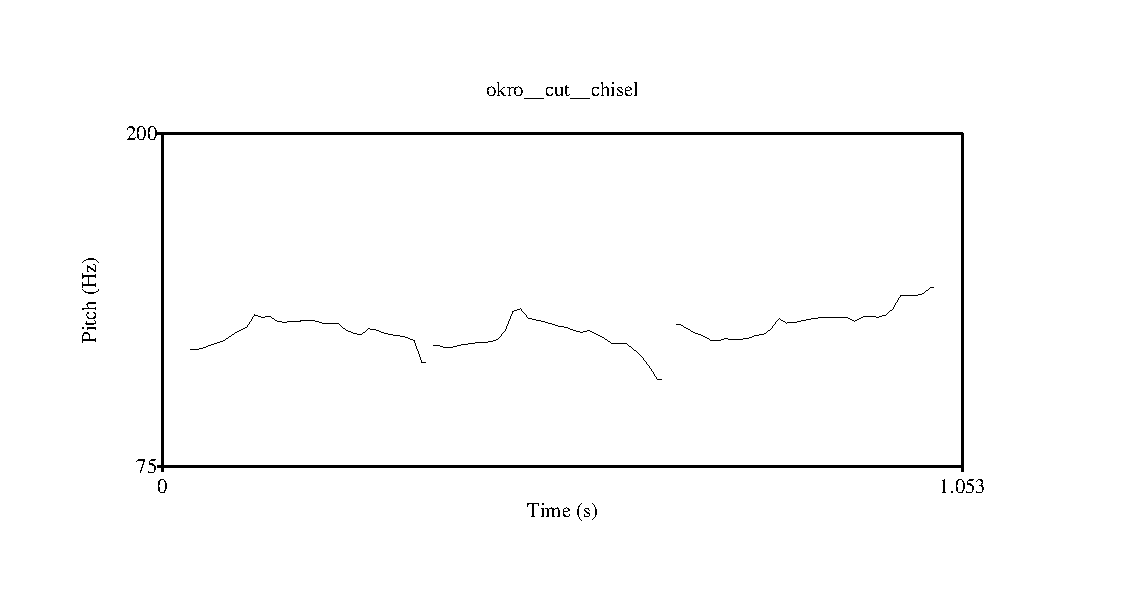
\includegraphics[width=11cm]{Graphic/Pictures/3sounds.pdf}
 \caption[Pitch contour of three words]{Pitch contour of the words for
 `okro', `to cut' and `chisel' (from left to right).  For each word, the contour
line starts at the beginning of the first consonant [ŋm] and  stops at the end
of the last vowel [a]. \label{fig:PHO-min-triplet}}
 \end{figure} 

% 
% \begin{figure}
% \centering
% 
%  \subfloat[][{\S ŋmɛ́ná}  `okro']{
% %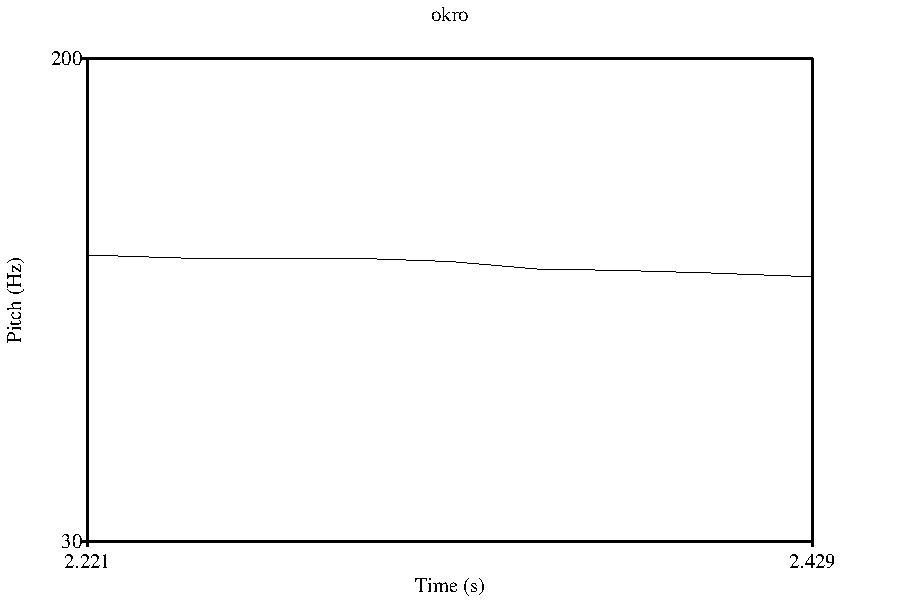
\includegraphics[width=5cm]{Graphic/Pictures/AD-okro.pdf}
%  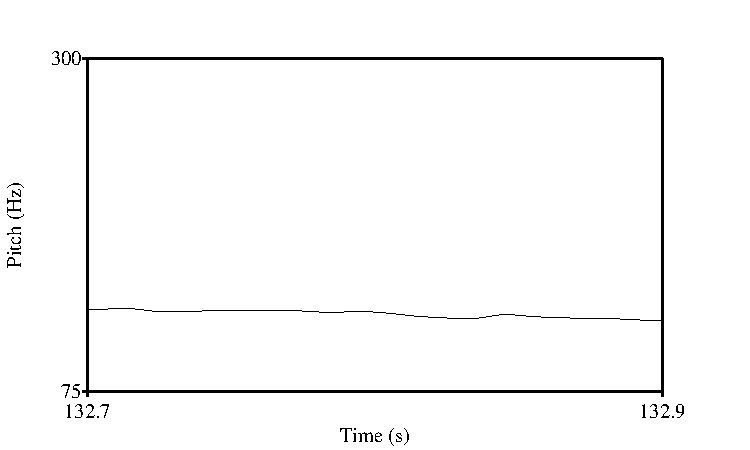
\includegraphics[width=5cm]{Graphic/Pictures/okro.pdf}
% }
% \qquad
%  \subfloat[][{\S ŋmɛ́nà} `cut']{
%  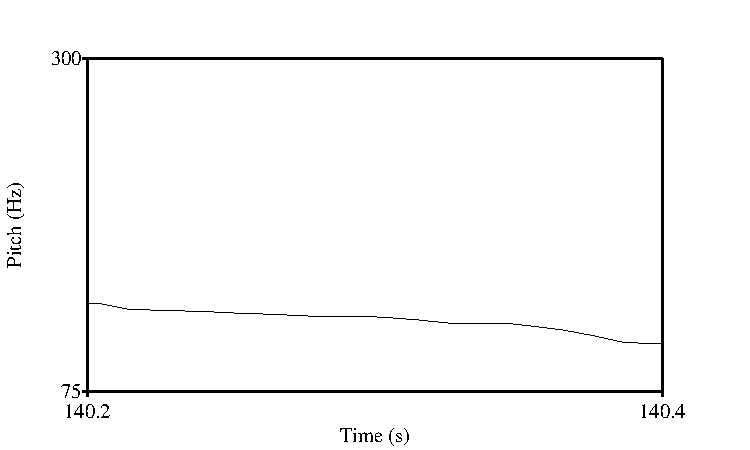
\includegraphics[width=5cm]{Graphic/Pictures/cut.pdf}
% }
% \qquad
%  \subfloat[][{\S ŋmɛ̀ná} `chisel']{
%  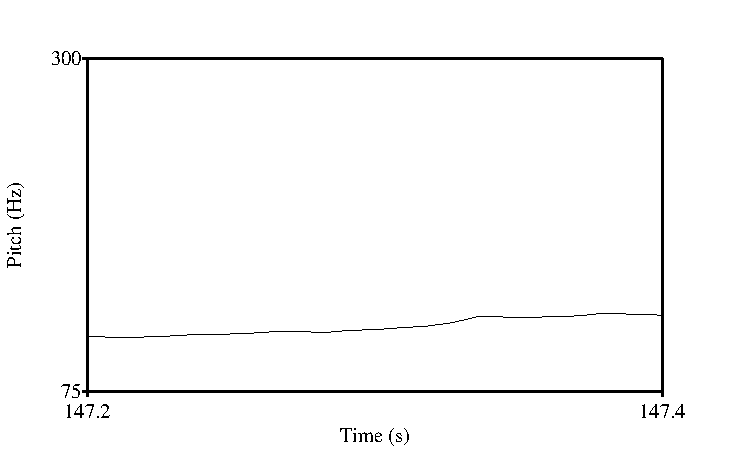
\includegraphics[width=5cm]{Graphic/Pictures/chisel.pdf}
% }
% 
% \caption[Pitch contours for three words]{Pitch contours of the words for
% `okro', `to cut' and `chisel'. Each window presents a time duration from the
% onset of the
% first vowel [ɛ] to the end of the last vowel [a]. 
% \label{fig:PHO-min-triplet}}
% 
% \end{figure} 

Distinct tonal melodies at the lexical level provide evidence that a pitch
distinction affects the meaning of words comprising identical sequences of
segments. The same can be said about tonal melodies at the phrasal level. Thus,
the sentences {\S ǹ̩ dí kʊ́ʊ́ rá} `I am eating t.z.' and {\S ǹ̩ dí kʊ̄ʊ̄
rā} `I ate t.z.' are composed of the same sequence of segments, but
it is mainly  the tonal
melody which distinguishes the former utterance from the latter.   Minimal
examples involving  specific tonal melodies are considered  in section
\ref{sec:GRM-trans-intran}.


Based on the evidence of nominal paradigms (see table \ref{tab:tone-sing-noun}),
 the evidence suggests there are two tones in the language, i.e. high (H) and
low (L).
They are transcribed on segments with an acute and a grave  accent respectively.
Since tones are assigned to moras, light syllables may get a single tone (i.e. H
or L). The heavy syllables may get high (H) or low (L), or either one of the
contour tones, i.e. falling (HL) or rising (LH). A mid tone is often perceived
but no contrast is found  at the lexical level. Provisionally,  the
mid tone is said to be a derived tone, that is, a raised low tone  or a lowered
high tone.
Table \ref{tab:tone-sing-noun} displays  the tonal melodies of the singular noun
category.  These are words uttered in isolation, so the tones are cut off from
contextual influences. The subtables are divided according to the 
moraic content of the syllable. As mentioned above, each mora is associated with
a single tone
and two tones are assumed. The  logical possibilities are accomodated with an
example.
%  The table
% \ref{tab:tone-sing-noun} is not exhaustive, other patterns exist.  
%downstepped hakila

\begin{table}[htp]
 %\centering
 \caption{Tonal patterns of singular nouns \label{tab:tone-sing-noun}}


\subfloat[][One light syllable CVC: non-moraic coda]{
\begin{Itabular}{llp{3.5cm}}
H& hóg	&	bone		\\
H& vʊ́g	&	small god\\	
L& bɔ̀g	&	type of tree	\\	
L& sʊ̀k	&	type of tree\\	
\end{Itabular}
}
\qquad
\subfloat[][One heavy syllable CVC: moraic coda]{
\begin{Itabular}{llp{3cm}}
H& 		kórː		&seat\\	
L &		sʊ̀lː		&dawadawa\\		
HL&		fʊ́l̀	&	type of creeper \\
LH& 	pòĺ		 & pond	 	\\
\end{Itabular}
}
\qquad
 \subfloat[][One heavy syllable CVVC]{
\begin{Itabular}{llp{3cm}}
H & fíél	&	type of grass\\
L & tʃʊ̀àr		& line	\\
HL & báàl	&	male	\\
LH & vàáŋ		& front leg	\\
\end{Itabular}
}
\qquad
\subfloat[][One heavy syllable CVV]{
\begin{Itabular}{llp{3cm}}
H&	bíí		& seed  \\
L&	 zùù	&	type of weather	\\	
HL&	lɔ́ʊ̀	& 	hartebeest	\\
LH&	 bìé	&  	child		\\
\end{Itabular}
}
\qquad
\subfloat[][Two light syllables CVCV]{
\begin{Itabular}{llp{3cm}}
  
H& bɪ́ná	& 	excrement	\\
L  & bɔ̀là		&elephant	\\
HL&	góŋò	 & 	type of tree	\\
LH & bɪ̀ná & 		year\\	
\end{Itabular}
}
\qquad
\subfloat[][One heavy CVC: non-moraic coda, one light]{
\begin{Itabular}{llp{3cm}}

H& tʃéllé		& outlaw	\\		
L & kpã̀nnà	&	lead\\
HL& dántà	&	clan title\\		
LH& kùksó	&	ribs	\\		
\end{Itabular}
}
\qquad
\subfloat[][One light CV, one heavy CVC]{
\begin{Itabular}{llp{3cm}}
H & búzóŋ	&	bachelor	\\
HL&  bʊ́zál̀ː	&	type of bird\\
LH & kàtʃíg	&	type of  bird\\
\end{Itabular}
}
\qquad
\subfloat[][One heavy CVV, one light CV]{
\begin{Itabular}{llp{3cm}}
 HHH & díésé & 		dream\\
HHL &  kpáásà	&	whip	\\
LHL & kùórù	&	chief	\\
LHH &	tùósó	&	added amount	\\
LLH &	fùòló	&	whistle	\\
LLL &	bʊ̀ɔ̀gà	&	moon	\\
\end{Itabular}
}
\qquad
\subfloat[][Three light syllables CVCVCV]{
\begin{Itabular}{llp{3cm}}

HHH &  kásɪ́má	&	corpse uniform	\\ 
HHL &  bélégè	& bathing area	\\
 LHL &  dùlúgù  &	type of bird \\
LLH &  gɛ̀rɛ̀gá	&	sickness\\
 LLL &  dɪ̀gɪ̀nà	&	ear	\\
 LLH &  tʃɪ̀rɪ̀bɔ́		&gun firing pin	\\
LHH &  ʔàmʊ́nʊ́	& 	type of wild cat\\ 
HLL &  kápùtì &  pillow \\

\end{Itabular}
}
\end{table}






% Tonal
% melodies in the verb phrase are presented in section \ref{}. Section \ref{}  
% will give an overview of the singular-plural tonal patterns in the noun
%classes.

These assumptions are not controversial: Vagla, Dɛg, Tampulma, Sisaala and
Pasaale are all described with two tones.\footnote{See \cite{Rowl65, Crou66,
Gray69,   Toup95, Crou03}.} One finds in this literature high and low tones and
a
considerable number of tone rules. Among them,  the
 downstep rule, aslo found in Chakali,   lowers a high tone (i.e. {\I ꜜ}H)  when
a
low tone intervenes between  two high tones, e.g. {\S dʊ̃́ʊ̃̀} ({\it sg.} HL), 
{\S dʊ̃́ꜜsá} 
({\it pl.} HLH). The rule in (\ref{PHO-downstep})
 captures the phenomenon. 


\begin{Rule}\label{PHO-downstep}{Downstep}\\
A high tone preceded by a low tone is perceived as lower than a preceding high
tone.\\
 H $>$  {\I ꜜ}H  / H  L \_
\end{Rule}

Downdrift is an intonation phenomenon: it is a
phrasal property by which a sequence of tones is cumulatively
lowered; underlyingly though, the tones are either high or low. This
gradual pitch fall may result in a low tone at the beginning of a phrase being 
as high as a high tone at the end of the phrase. Example
(\ref{exːPHO-downdrift}) illustrates the
phenomenon. While the first line shows how the tones are perceived, the second
line provides the lexical  tones normally associated with each of the
words.\footnote{The lack of tone rules in the  description is an important 
level of analysis lacking between phrasal intonation and lexical tones,  so
example 
(\ref{exːPHO-downdrift}) must be interpreted with vigilance.}


\begin{exe}
\ex\label{exːPHO-downdrift}

\glll {\T } {\T } {\T  } {\T } {\T }\\
váà tʃʊ̀á dɪ̀á nʊ̀ã́ nɪ́ \\
dog lie house mouth {\postp} \\
\glt  `A dog lies at the entrance of a house.'
\end{exe}


\begin{Rule}\label{PHO-polar-drop}{Polar question drop}\\
A tone (or a series of tones) changes into an extra-low tone at an
utterance-final boundary (condition:  polar question).\\
H*|L*  $>$  XL  /  \_ \#\#
\end{Rule}



Generally seen as a discourse function, Chakali has an extra-low tone  which
appears at the end of  polar question (see section
\ref{sec:GRM-interr-polar}). It is marked with
the diacritic [v̏]. 
Rule \ref{PHO-polar-drop} describes the intonation (drop of pitch) of  polar
questions.
%see Gussenhoven for superlow


%\subsection{Tone-bearing unit}
%\subsection{Underlying tone}
%\subsection{Tone perturbation}





\subsection{Vowel Harmony}
\label{sec:vowel-harmony}

Vowel harmony is a process in  which all the vowels in a particular domain come
to share one or more phonological feature(s).   This agreement  is
triggered in specific phonological domains, usually the word, and  has a
particular direction which is often treated as the spreading of one or more
vowel feature(s). 

In section \ref{sec:vowels},  evidence was provided for the establishment of
nine
underlying vowels with five {\sc -atr} and four  {\sc +atr} vowels. This
type of  vowel inventory has been referred to as  a five-height (5Ht) system 
\citep[308]{Casa03},  in which the
feature {\sc atr} is contrastive within both the {\sc +hi} and {\sc [-hi,
-lo]} vowels (see table \ref{tab:featspec}).  \citet[81-82]{Daku97} and
\citet[312]{Casa03} maintain that it is the most common inventory among
Gur and Kwa languages. 


In section \ref{sec:LOW-phon-vowel},  the
{\sc -atr} specification of the low vowel at the phonemic level was assumed
  on the basis of its behavior with the set of {\sc -atr} vowels. In
fact, the  realization of the low vowel in vowel harmony suggests that the set
of vowels specified as {\sc -atr}  contains the low vowel. To illustrate
the properties of vowel harmony, let us consider
how they function in  monosyllabic noun roots. Consider the data in
table
\ref{tab:examples-harmony}.



\begin{table}[!htb]
\centering
\caption{Vowel harmony in noun words\label{tab:examples-harmony}}
 \begin{tabular}{lllll}
\Hline
Root vowel feature & Root &  Singular & Plural & Gloss\\ \hline

{\sc [+atr, +mid, -ro]} &sel& sélː&sélé & animal\\
{\sc [+atr, +hi, -ro]} &bi &bíí &bíé& seed \\
{\sc [+atr, -ro]} &kie&  kìé 	&kìété	&half of a bird\\
{\sc [+atr, +hi, +ro]} &ʔul & ʔúl 	& ʔúló 	  & 	navel\\
{\sc [+atr, +mid, +ro]} &hol& hól & hóló & type of tree   \\
{\sc [+atr, +ro]} &buo& bùó 	& bùósó  &	funeral item\\
{\sc [-atr, +hi, -ro]} &bɪ& bɪ́ɪ́	&	bɪ́á 		&	stone\\
{\sc [-atr, +mid, -ro]} &bɛl & bɛ̀ĺ &bɛ́llá & type of tree \\
{\sc [-atr, +hi, +ro]} & ɲʊg& ɲʊ́g & ɲʊ́gá & crocodile \\
{\sc [-atr, +mid, +ro]} & hɔl& hɔ́l & hɔ́lá & piece of charcoal  \\
{\sc [-atr, +ro]} & bʊɔ& bʊ̀ɔ́	& bʊ̀ɔ̀sá	  &	hole\\
{\sc [-atr, +lo]} &vaa& váá  & vásá & dog \\
{\sc [-atr, +lo]} &baal& báàl& báàlá& male \\

  \Hline
 \end{tabular}

\end{table}  

 Chakali is a language with
noun classes (see section \ref{sec:GRM-noun-classes}). A class is defined as a
pair of singular and plural suffixes
associated with
a particular root.  Looking first at the plural noun endings in table
\ref{tab:examples-harmony}, it seems that from the underlying nine vowel
inventory of Chakali, only three can occur in such a position, i.e. {\S -a}, {\S
-e} and {\S -o}. The distribution is such that  when the suffixes occur after a
root containing any member of the set \{ɪ, ɛ, ɔ, ʊ, a\},  they are realized as
[-a].  The plural suffix vowel {\S e} is realized when the root features are
{\sc [+atr, -ro]}, whereas the plural suffix vowel {\S o} is realized when the
root features are {\sc [+atr, +ro]}.  Notice that the height feature(s) of a
vowel is irrelevant in all cases.  Rules \ref{RULE-nc-rule-1} and
\ref{RULE-nc-rule-2} accomodate the surface forms of table
\ref{tab:examples-harmony}.\footnote{\citet[19, 32-33]{Okee03} states that {\sc
ro}- and {\sc atr}-harmony are both operative in the progressive, future,
egressive and ingressive of Fante.}


\begin{Rule}\label{RULE-nc-rule-1}{Noun classes realization (1)}\\
A noun class suffix vowel becomes {\sc +atr} if preceded by a {\sc +atr}
stem vowel, and shares the same value for the
feature {\sc ro}  as the one specified on the preceding stem vowel. \\
-V_{nc} $>$ [ $\beta${\sc ro},  {\sc +atr}, {\sc +mid}]  / [ $\beta${\sc ro},
{\sc +atr}] C* \_

\end{Rule}


\begin{Rule}\label{RULE-nc-rule-2}{Noun classes realization (2)}\\
A noun class suffix vowel becomes {\S a} if the preceding stem vowel is 
{\S ɪ},
{\S ɛ}, {\S ɔ}, {\S ʊ} or {\S a}.\\
-V_{nc} $>$ {\sc +lo}  / {\sc -atr} C* \_ 
\end{Rule}


The same rules may be used to account for the vowel
quality of the focus marker (section \ref{sec:focus-forms}) and  the verbal
suffixes (section \ref{sec:nasalization-verb-suffix}). Yet, the rules need to
be rewritten in order to be  applicable to wider domains and elements than
those defined in their definition. Rules \ref{RULE-atr} and \ref{RULE-ro} break
down rules \ref{RULE-nc-rule-1} and \ref{RULE-nc-rule-2} into components able to
be applied to other relevant domains.



\begin{Rule}\label{RULE-atr}{{\sc atr} harmony}\\
A vowel suffix agrees with the {\sc atr} value of   the preceding stem/word 
vowel (domains: noun classes, verbal suffixes, focus marker).\\
V $>$ $[\alpha${\sc atr}$]$  / $[\alpha${\sc atr}$]$ C* \_
\end{Rule}


\begin{Rule}\label{RULE-ro}{{\sc ro} harmony}\\
A vowel suffix  agree with the {\sc ro} value of  the   preceding stem/word
 vowel (domains: noun classes, verbal suffixes, focus marker).\\
V $>$ [$\alpha${\sc ro}]  / [$\alpha${\sc ro}] C* \_
\end{Rule}

Up to the present, the data suggest that the low vowel is excluded from
co-occurring with {\sc +atr}  vowels.  So the prediction seems to be that if a
word contains a {\sc +atr} vowel,  either the low vowel {\I /a/} cannot be
realized and is thus changed by (one of) the above rules, or  the  low vowel {\I
/a/} is banned  altogether from the underlying form. Caution is necessary
however since complex stem nouns (section \ref{sec:GRM-com-stem-noun}) are
attested containing both  low vowels and {\sc +atr} vowels, e.g. {\S pàzèŋ́}
($<$ {\S par-zeŋ}, {\sc hoe-big})  `big hoe'. Moreover, some multisyllabic words
which cannot be treated as complex stem nouns due to their lack of morphological
transparency do appear with both  a {\sc +atr} vowel and  the low vowel. The
phonological and/or morphological domains where one could draw the line are
still undetermined.


